\PassOptionsToPackage{unicode=true}{hyperref} % options for packages loaded elsewhere
\PassOptionsToPackage{hyphens}{url}
%
\documentclass[11pt,ignorenonframetext,]{beamer}
\usepackage{pgfpages}
\setbeamertemplate{caption}[numbered]
\setbeamertemplate{caption label separator}{: }
\setbeamercolor{caption name}{fg=normal text.fg}
\beamertemplatenavigationsymbolsempty
% Prevent slide breaks in the middle of a paragraph:
\widowpenalties 1 10000
\raggedbottom
\setbeamertemplate{part page}{
\centering
\begin{beamercolorbox}[sep=16pt,center]{part title}
  \usebeamerfont{part title}\insertpart\par
\end{beamercolorbox}
}
\setbeamertemplate{section page}{
\centering
\begin{beamercolorbox}[sep=12pt,center]{part title}
  \usebeamerfont{section title}\insertsection\par
\end{beamercolorbox}
}
\setbeamertemplate{subsection page}{
\centering
\begin{beamercolorbox}[sep=8pt,center]{part title}
  \usebeamerfont{subsection title}\insertsubsection\par
\end{beamercolorbox}
}
\AtBeginPart{
  \frame{\partpage}
}
\AtBeginSection{
  \ifbibliography
  \else
    \frame{\sectionpage}
  \fi
}
\AtBeginSubsection{
  \frame{\subsectionpage}
}
\usepackage{lmodern}
\usepackage{amssymb,amsmath}
\usepackage{ifxetex,ifluatex}
\usepackage{fixltx2e} % provides \textsubscript
\ifnum 0\ifxetex 1\fi\ifluatex 1\fi=0 % if pdftex
  \usepackage[T1]{fontenc}
  \usepackage[utf8]{inputenc}
  \usepackage{textcomp} % provides euro and other symbols
\else % if luatex or xelatex
  \usepackage{unicode-math}
  \defaultfontfeatures{Ligatures=TeX,Scale=MatchLowercase}
\fi
\usetheme[]{metropolis}
% use upquote if available, for straight quotes in verbatim environments
\IfFileExists{upquote.sty}{\usepackage{upquote}}{}
% use microtype if available
\IfFileExists{microtype.sty}{%
\usepackage[]{microtype}
\UseMicrotypeSet[protrusion]{basicmath} % disable protrusion for tt fonts
}{}
\IfFileExists{parskip.sty}{%
\usepackage{parskip}
}{% else
\setlength{\parindent}{0pt}
\setlength{\parskip}{6pt plus 2pt minus 1pt}
}
\usepackage{hyperref}
\hypersetup{
            pdftitle={Lecture 18},
            pdfauthor={Colin Rundel},
            pdfborder={0 0 0},
            breaklinks=true}
\urlstyle{same}  % don't use monospace font for urls
\newif\ifbibliography
\usepackage{color}
\usepackage{fancyvrb}
\newcommand{\VerbBar}{|}
\newcommand{\VERB}{\Verb[commandchars=\\\{\}]}
\DefineVerbatimEnvironment{Highlighting}{Verbatim}{commandchars=\\\{\}}
% Add ',fontsize=\small' for more characters per line
\newenvironment{Shaded}{}{}
\newcommand{\AlertTok}[1]{\textcolor[rgb]{1.00,0.00,0.00}{\textbf{#1}}}
\newcommand{\AnnotationTok}[1]{\textcolor[rgb]{0.38,0.63,0.69}{\textbf{\textit{#1}}}}
\newcommand{\AttributeTok}[1]{\textcolor[rgb]{0.49,0.56,0.16}{#1}}
\newcommand{\BaseNTok}[1]{\textcolor[rgb]{0.25,0.63,0.44}{#1}}
\newcommand{\BuiltInTok}[1]{#1}
\newcommand{\CharTok}[1]{\textcolor[rgb]{0.25,0.44,0.63}{#1}}
\newcommand{\CommentTok}[1]{\textcolor[rgb]{0.38,0.63,0.69}{\textit{#1}}}
\newcommand{\CommentVarTok}[1]{\textcolor[rgb]{0.38,0.63,0.69}{\textbf{\textit{#1}}}}
\newcommand{\ConstantTok}[1]{\textcolor[rgb]{0.53,0.00,0.00}{#1}}
\newcommand{\ControlFlowTok}[1]{\textcolor[rgb]{0.00,0.44,0.13}{\textbf{#1}}}
\newcommand{\DataTypeTok}[1]{\textcolor[rgb]{0.56,0.13,0.00}{#1}}
\newcommand{\DecValTok}[1]{\textcolor[rgb]{0.25,0.63,0.44}{#1}}
\newcommand{\DocumentationTok}[1]{\textcolor[rgb]{0.73,0.13,0.13}{\textit{#1}}}
\newcommand{\ErrorTok}[1]{\textcolor[rgb]{1.00,0.00,0.00}{\textbf{#1}}}
\newcommand{\ExtensionTok}[1]{#1}
\newcommand{\FloatTok}[1]{\textcolor[rgb]{0.25,0.63,0.44}{#1}}
\newcommand{\FunctionTok}[1]{\textcolor[rgb]{0.02,0.16,0.49}{#1}}
\newcommand{\ImportTok}[1]{#1}
\newcommand{\InformationTok}[1]{\textcolor[rgb]{0.38,0.63,0.69}{\textbf{\textit{#1}}}}
\newcommand{\KeywordTok}[1]{\textcolor[rgb]{0.00,0.44,0.13}{\textbf{#1}}}
\newcommand{\NormalTok}[1]{#1}
\newcommand{\OperatorTok}[1]{\textcolor[rgb]{0.40,0.40,0.40}{#1}}
\newcommand{\OtherTok}[1]{\textcolor[rgb]{0.00,0.44,0.13}{#1}}
\newcommand{\PreprocessorTok}[1]{\textcolor[rgb]{0.74,0.48,0.00}{#1}}
\newcommand{\RegionMarkerTok}[1]{#1}
\newcommand{\SpecialCharTok}[1]{\textcolor[rgb]{0.25,0.44,0.63}{#1}}
\newcommand{\SpecialStringTok}[1]{\textcolor[rgb]{0.73,0.40,0.53}{#1}}
\newcommand{\StringTok}[1]{\textcolor[rgb]{0.25,0.44,0.63}{#1}}
\newcommand{\VariableTok}[1]{\textcolor[rgb]{0.10,0.09,0.49}{#1}}
\newcommand{\VerbatimStringTok}[1]{\textcolor[rgb]{0.25,0.44,0.63}{#1}}
\newcommand{\WarningTok}[1]{\textcolor[rgb]{0.38,0.63,0.69}{\textbf{\textit{#1}}}}
\setlength{\emergencystretch}{3em}  % prevent overfull lines
\providecommand{\tightlist}{%
  \setlength{\itemsep}{0pt}\setlength{\parskip}{0pt}}
\setcounter{secnumdepth}{0}

% set default figure placement to htbp
\makeatletter
\def\fps@figure{htbp}
\makeatother

\usepackage{geometry}
\usepackage{graphicx}

\usepackage{bbold}
\usepackage{lmodern}


\usepackage{url}		% produces hyperlinks

\usepackage{colortbl}	% allows for color usage in tables
\usepackage{multirow}	% allows for rows that span multiple rows in tables

\usepackage{color}          	% gives color options
\usepackage{xcolor}		% this package has a variety of color options

\usepackage{multicol}
\usepackage{textcomp}

\usepackage{setspace}
\usepackage{changepage}
\usepackage{isotope}

\singlespacing

\def\begincol{\begin{column}}
\def\endcol{\end{column}}

\def\begincols{\begin{columns}}
\def\endcols{\end{columns}}

%%%%%%%%%%%%%%%%
% Small code output
%%%%%%%%%%%%%%%%

%% change fontsize of R code

\makeatletter
\@ifundefined{Shaded}{\newenvironment{Shaded}{}{}}{}
\makeatother


\let\oldShaded\Shaded
\let\endoldShaded\endShaded
\renewenvironment{Shaded}{\footnotesize\begin{spacing}{0.9}\oldShaded}{\endoldShaded\end{spacing}}

%% change fontsize of output
\let\oldverbatim\verbatim
\let\endoldverbatim\endverbatim
\renewenvironment{verbatim}{\footnotesize\begin{spacing}{0.9}\oldverbatim}{\endoldverbatim\end{spacing}}


\newcommand{\tinyoutput}{
  \renewenvironment{Shaded}{\tiny\begin{spacing}{0.9}\oldShaded}{\endoldShaded\end{spacing}}
  \renewenvironment{verbatim}{\tiny\begin{spacing}{0.9}\oldverbatim}{\endoldverbatim\end{spacing}}
}

\newcommand{\scriptoutput}{
  \renewenvironment{Shaded}{\scriptsize\begin{spacing}{0.9}\oldShaded}{\endoldShaded\end{spacing}}
  \renewenvironment{verbatim}{\scriptsize\begin{spacing}{0.9}\oldverbatim}{\endoldverbatim\end{spacing}}
}

\newcommand{\footnoteoutput}{
  \renewenvironment{Shaded}{\footnotesize\begin{spacing}{0.9}\oldShaded}{\endoldShaded\end{spacing}}
  \renewenvironment{verbatim}{\footnotesize\begin{spacing}{0.9}\oldverbatim}{\endoldverbatim\end{spacing}}
}

%\newcommand{\verbatimfont}[1]{\renewcommand{\verbatim@font}{\ttfamily#1}}


%%%%%%%%%%%%%%%%
% Custom Colors
%%%%%%%%%%%%%%%%

\definecolor{redhl}{rgb}{0.98,0.29,0.28}
\definecolor{yellowhl}{rgb}{0.98,0.87,0.28}


\xdefinecolor{oiBlue}{rgb}{0.15, 0.35, 0.55}
\xdefinecolor{gray}{rgb}{0.5, 0.5, 0.5}
\xdefinecolor{darkGray}{rgb}{0.3, 0.3, 0.3}
\xdefinecolor{darkerGray}{rgb}{0.2, 0.2, 0.2}
\xdefinecolor{rubineRed}{rgb}{0.89,0,0.30}
\xdefinecolor{linkCol}{rgb}{0.11,0.49,0.95}	
\xdefinecolor{irishGreen}{rgb}{0,0.60,0}	
\xdefinecolor{darkturquoise}{rgb}{0.44, 0.58, 0.86}
\definecolor{lightGreen}{rgb}{0.533,0.765,0.42}
%\xdefinecolor{hlblue}{rgb}{0.051,0.65,1}
\xdefinecolor{hlblue}{rgb}{ 0.055, 0.639, 0.831}
\definecolor{light}{rgb}{.337,.608,.741}
\definecolor{dark}{rgb}{.337,.608,.741}

\definecolor{cpink}{rgb}{0.93, 0.23, 0.51}

%%%%%%%%%%%%%%%%
% Custom Commands
%%%%%%%%%%%%%%%%

% text colors
\newcommand{\red}[1]{\textit{\textcolor{rubineRed}{#1}}}
\newcommand{\orange}[1]{\textit{\textcolor{orange}{#1}}}
\newcommand{\pink}[1]{\textit{\textcolor{rubineRed!90!white!50}{#1}}}
\newcommand{\green}[1]{\textit{\textcolor{irishGreen}{#1}}}
\newcommand{\blue}[1]{\textit{\textcolor{darkturquoise}{#1}}}
\newcommand{\light}[1]{\textcolor{light}{\textbf{#1}}}
\newcommand{\dark}[1]{\textcolor{dark}{#1}}
\newcommand{\gray}[1]{\textcolor{gray}{#1}}


% mail
\newcommand{\mail}[1]{\href{mailto:#1}{\textit{\textcolor{linkCol}{#1}}}}

% highlighting: hl, hlGr, mathhl
\newcommand{\hl}[1]{\textit{\textcolor{hlblue}{#1}}}
\newcommand{\hlGr}[1]{\textit{\textcolor{lightGreen}{#1}}}
\newcommand{\hlRd}[1]{\textit{\textcolor{rubineRed}{#1}}}
\newcommand{\mathhl}[1]{\textcolor{hlblue}{\ensuremath{#1}}}
\newcommand{\hlr}[1]{\fcolorbox{redhl}{white}{$\displaystyle #1$}}
\newcommand{\hly}[1]{\fcolorbox{yellowhl}{white}{$\displaystyle #1$}}


\newcommand{\vvfill}{\vskip0pt plus 1filll}

\DeclareMathOperator*{\argmin}{arg\,min}
\DeclareMathOperator*{\argmax}{arg\,max}

\title{Lecture 18}
\providecommand{\subtitle}[1]{}
\subtitle{Fitting CAR and SAR Models}
\author{Colin Rundel}
\date{11/07/2018}

\begin{document}
\frame{\titlepage}

\hypertarget{fitting-areal-models}{%
\section{Fitting areal models}\label{fitting-areal-models}}

\begin{frame}[t]{Revised SAR Model}
\protect\hypertarget{revised-sar-model}{}

\begin{itemize}
\tightlist
\item
  Formula Model
\end{itemize}

\[ y(s_i) = X_{i\cdot}\beta + \phi \sum_{j=1}^n D^{-1}_{jj} \, A_{ij} \, \big(y(s_j) - X_{j\cdot}\beta\big) + \epsilon_i \]
\[ \symbf{\epsilon} \sim \mathcal{N}(\symbf{0},\, \sigma^2 \symbf{D}^{-1}) \]

\begin{itemize}
\tightlist
\item
  Joint Model
\end{itemize}

\[
\symbf{y} \sim \mathcal{N}\left(\symbf{X}\symbf{\beta}, (\symbf{I} - \phi \symbf{D}^{-1} \symbf{A})^{-1} \sigma^2 \symbf{D}^{-1} \big((\symbf{I} - \phi \symbf{D}^{-1} \symbf{A})^{-1}\big)^t \right)
\]

\end{frame}

\begin{frame}[t]{Revised CAR Model}
\protect\hypertarget{revised-car-model}{}

\begin{itemize}
\tightlist
\item
  Conditional Model
\end{itemize}

\[ y(s_i)|\symbf{y}_{-s_i} \sim \mathcal{N}\left(X_{i\cdot}\beta + \phi\sum_{j=1}^n \frac{A_{ij}}{D_{ii}} ~ \big(y(s_j)-X_{j\cdot}\beta\big),~ \sigma^2 D^{-1}_{ii} \right) \]

\begin{itemize}
\tightlist
\item
  Joint Model
\end{itemize}

\[\symbf{y} \sim \mathcal{N}(\symbf{X}\symbf{\beta},~\sigma^2(\symbf{D}-\phi \symbf{A})^{-1})\]

\end{frame}

\begin{frame}{Example - NC SIDS}
\protect\hypertarget{example---nc-sids}{}

\begin{center}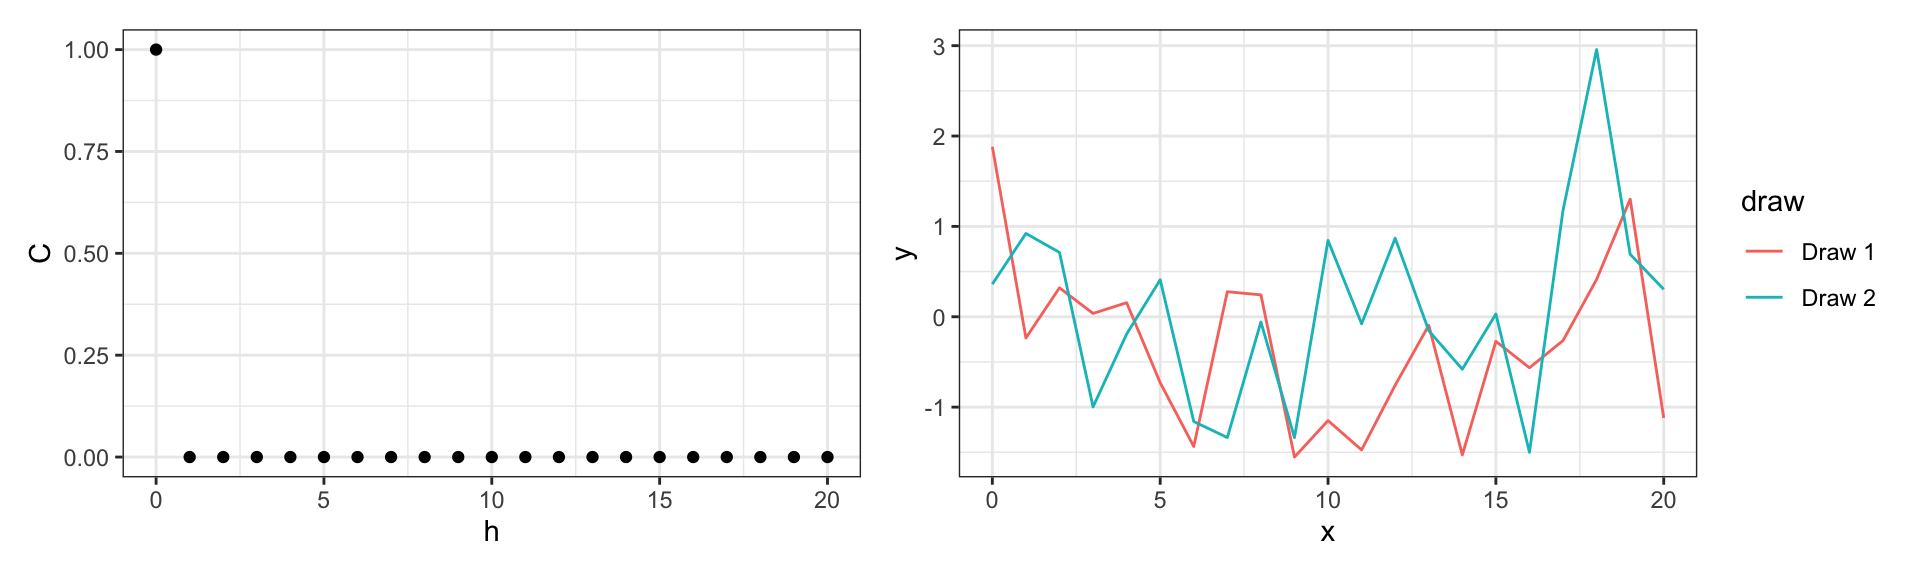
\includegraphics[width=\textwidth]{Lec18_files/figure-beamer/unnamed-chunk-1-1} \end{center}

\end{frame}

\begin{frame}[fragile]{}
\protect\hypertarget{section}{}

\begin{Shaded}
\begin{Highlighting}[]
\KeywordTok{ggplot}\NormalTok{() }\OperatorTok{+}\StringTok{ }\KeywordTok{geom_sf}\NormalTok{(}\DataTypeTok{data=}\NormalTok{nc, }\KeywordTok{aes}\NormalTok{(}\DataTypeTok{fill=}\NormalTok{SID74}\OperatorTok{/}\NormalTok{BIR74}\OperatorTok{*}\DecValTok{1000}\NormalTok{))}
\end{Highlighting}
\end{Shaded}

\begin{center}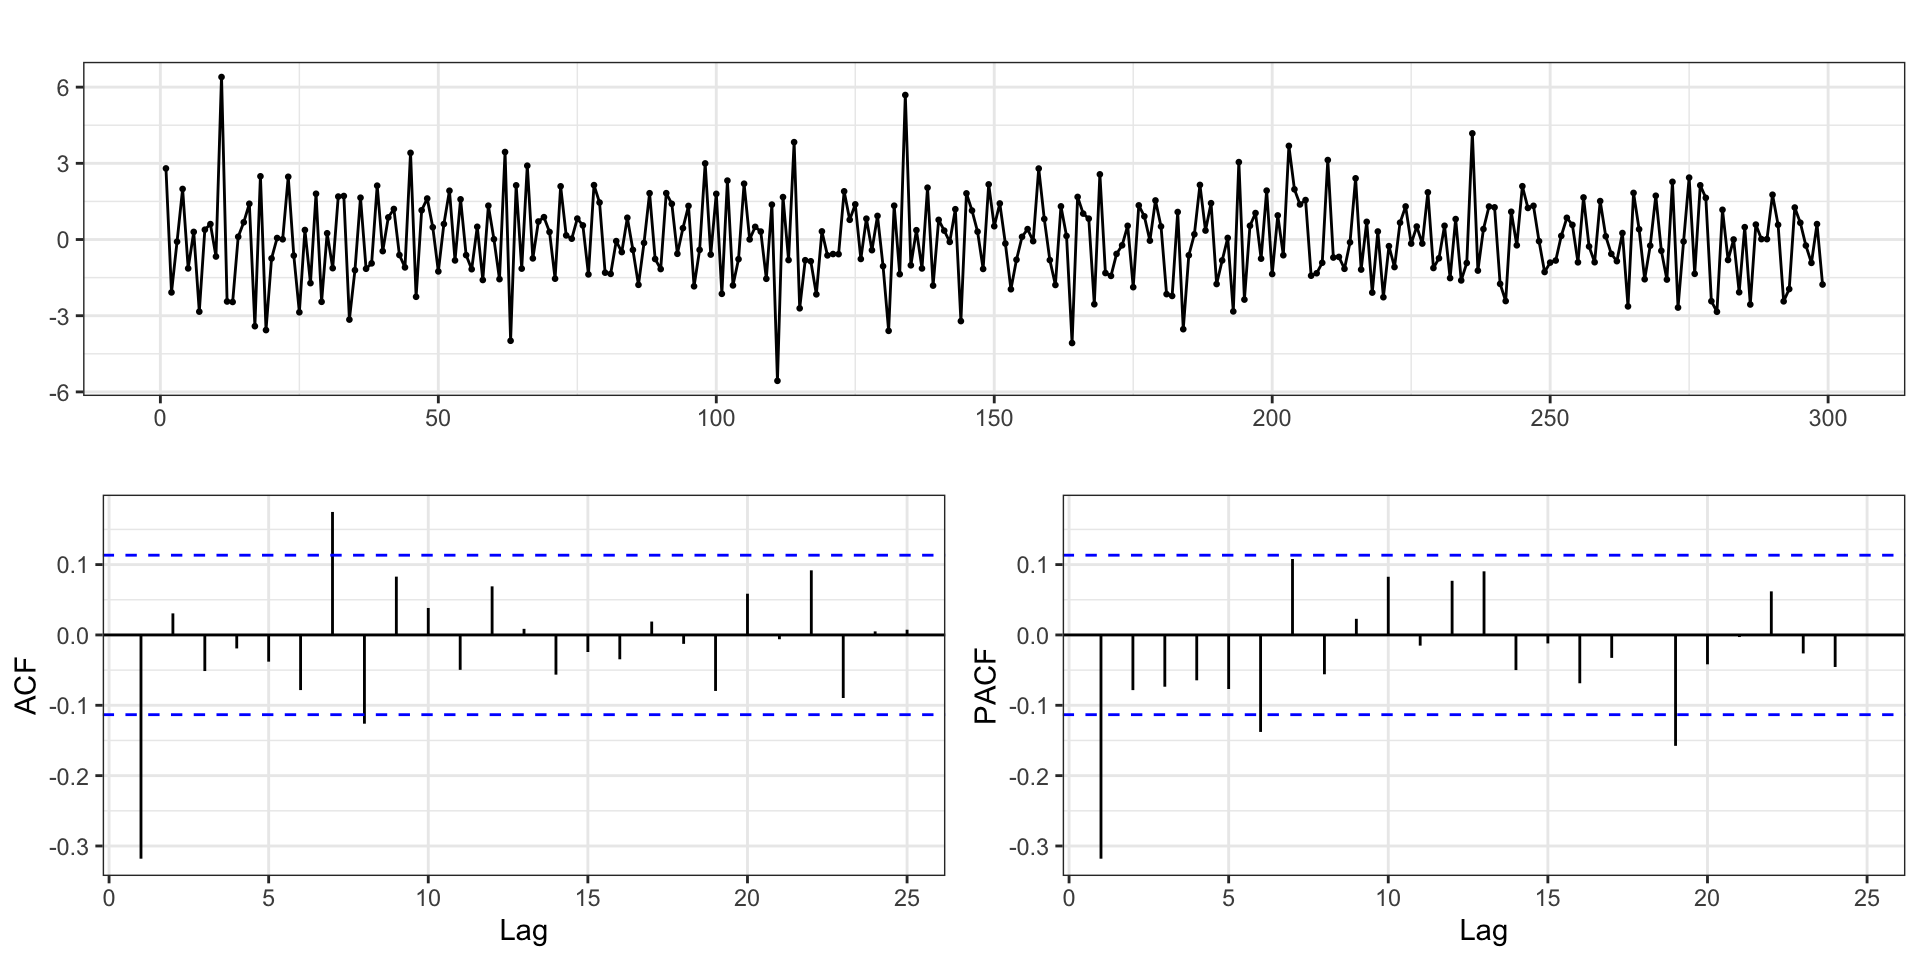
\includegraphics[width=\textwidth]{Lec18_files/figure-beamer/unnamed-chunk-2-1} \end{center}

\end{frame}

\begin{frame}[fragile,t]{Using \texttt{spautolm} from \texttt{spdep}}
\protect\hypertarget{using-spautolm-from-spdep}{}

\begin{Shaded}
\begin{Highlighting}[]
\KeywordTok{library}\NormalTok{(spdep)}

\NormalTok{A =}\StringTok{ }\KeywordTok{st_touches}\NormalTok{(nc, }\DataTypeTok{sparse=}\OtherTok{FALSE}\NormalTok{)}
\NormalTok{listW =}\StringTok{ }\KeywordTok{mat2listw}\NormalTok{(A)}

\NormalTok{listW}
\CommentTok{## Characteristics of weights list object:}
\CommentTok{## Neighbour list object:}
\CommentTok{## Number of regions: 100 }
\CommentTok{## Number of nonzero links: 490 }
\CommentTok{## Percentage nonzero weights: 4.9 }
\CommentTok{## Average number of links: 4.9 }
\CommentTok{## }
\CommentTok{## Weights style: M }
\CommentTok{## Weights constants summary:}
\CommentTok{##     n    nn  S0  S1    S2}
\CommentTok{## M 100 10000 490 980 10696}
\end{Highlighting}
\end{Shaded}

\end{frame}

\begin{frame}[fragile,t]{}
\protect\hypertarget{section-1}{}

\begin{Shaded}
\begin{Highlighting}[]
\NormalTok{nc_coords =}\StringTok{ }\NormalTok{nc }\OperatorTok\StringTok{ }\KeywordTok{st_centroid}\NormalTok{() }\OperatorTok\StringTok{ }\KeywordTok{st_coordinates}\NormalTok{()}

\KeywordTok{plot}\NormalTok{(}\KeywordTok{st_geometry}\NormalTok{(nc))}
\KeywordTok{plot}\NormalTok{(listW, nc_coords, }\DataTypeTok{add=}\OtherTok{TRUE}\NormalTok{, }\DataTypeTok{col=}\StringTok{"blue"}\NormalTok{, }\DataTypeTok{pch=}\DecValTok{16}\NormalTok{)}
\end{Highlighting}
\end{Shaded}

\begin{center}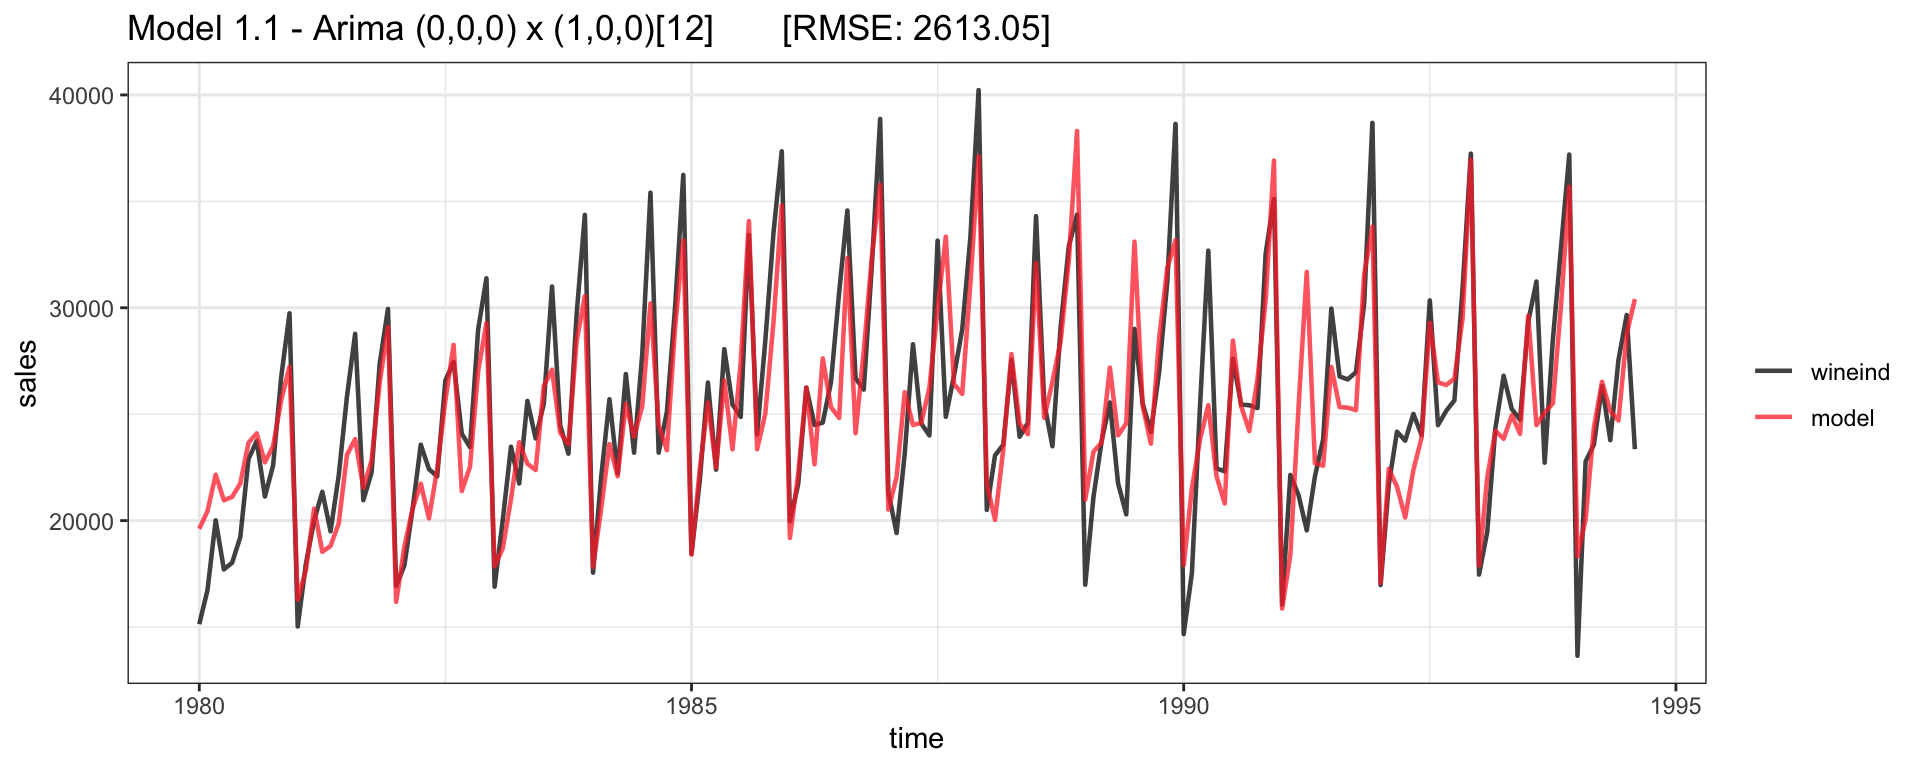
\includegraphics[width=\textwidth]{Lec18_files/figure-beamer/unnamed-chunk-4-1} \end{center}

\end{frame}

\begin{frame}[fragile]{Moran's I}
\protect\hypertarget{morans-i}{}

\footnotesize

\begin{Shaded}
\begin{Highlighting}[]
\NormalTok{spdep}\OperatorTok{::}\KeywordTok{moran.test}\NormalTok{(nc}\OperatorTok{$}\NormalTok{SID74, listW)}
\CommentTok{## }
\CommentTok{##  Moran I test under randomisation}
\CommentTok{## }
\CommentTok{## data:  nc$SID74  }
\CommentTok{## weights: listW    }
\CommentTok{## }
\CommentTok{## Moran I statistic standard deviate = 2.1707, p-value = 0.01498}
\CommentTok{## alternative hypothesis: greater}
\CommentTok{## sample estimates:}
\CommentTok{## Moran I statistic       Expectation          Variance }
\CommentTok{##       0.119089049      -0.010101010       0.003542176}
\NormalTok{spdep}\OperatorTok{::}\KeywordTok{moran.test}\NormalTok{(}\DecValTok{1000}\OperatorTok{*}\NormalTok{nc}\OperatorTok{$}\NormalTok{SID74}\OperatorTok{/}\NormalTok{nc}\OperatorTok{$}\NormalTok{BIR74, listW)}
\CommentTok{## }
\CommentTok{##  Moran I test under randomisation}
\CommentTok{## }
\CommentTok{## data:  1000 * nc$SID74/nc$BIR74  }
\CommentTok{## weights: listW    }
\CommentTok{## }
\CommentTok{## Moran I statistic standard deviate = 3.6355, p-value = 0.0001387}
\CommentTok{## alternative hypothesis: greater}
\CommentTok{## sample estimates:}
\CommentTok{## Moran I statistic       Expectation          Variance }
\CommentTok{##       0.210046454      -0.010101010       0.003666802}
\end{Highlighting}
\end{Shaded}

\end{frame}

\begin{frame}[fragile]{Geary's C}
\protect\hypertarget{gearys-c}{}

\begin{Shaded}
\begin{Highlighting}[]
\NormalTok{spdep}\OperatorTok{::}\KeywordTok{geary.test}\NormalTok{(nc}\OperatorTok{$}\NormalTok{SID74, listW)}
\CommentTok{## }
\CommentTok{##  Geary C test under randomisation}
\CommentTok{## }
\CommentTok{## data:  nc$SID74 }
\CommentTok{## weights: listW }
\CommentTok{## }
\CommentTok{## Geary C statistic standard deviate = 0.91949, p-value = 0.1789}
\CommentTok{## alternative hypothesis: Expectation greater than statistic}
\CommentTok{## sample estimates:}
\CommentTok{## Geary C statistic       Expectation          Variance }
\CommentTok{##        0.88988684        1.00000000        0.01434105}
\NormalTok{spdep}\OperatorTok{::}\KeywordTok{geary.test}\NormalTok{(nc}\OperatorTok{$}\NormalTok{SID74}\OperatorTok{/}\NormalTok{nc}\OperatorTok{$}\NormalTok{BIR74, listW)}
\CommentTok{## }
\CommentTok{##  Geary C test under randomisation}
\CommentTok{## }
\CommentTok{## data:  nc$SID74/nc$BIR74 }
\CommentTok{## weights: listW }
\CommentTok{## }
\CommentTok{## Geary C statistic standard deviate = 3.0989, p-value = 0.0009711}
\CommentTok{## alternative hypothesis: Expectation greater than statistic}
\CommentTok{## sample estimates:}
\CommentTok{## Geary C statistic       Expectation          Variance }
\CommentTok{##        0.67796679        1.00000000        0.01079878}
\end{Highlighting}
\end{Shaded}

\end{frame}

\begin{frame}[fragile,t]{CAR Model}
\protect\hypertarget{car-model}{}

\scriptoutput

\begin{Shaded}
\begin{Highlighting}[]
\NormalTok{nc_car =}\StringTok{ }\KeywordTok{spautolm}\NormalTok{(}\DataTypeTok{formula =}\NormalTok{ SID74}\OperatorTok{/}\NormalTok{BIR74 }\OperatorTok{~}\StringTok{ }\DecValTok{1}\NormalTok{, }\DataTypeTok{data =}\NormalTok{ nc, }
                  \DataTypeTok{listw =}\NormalTok{ listW, }\DataTypeTok{family =} \StringTok{"CAR"}\NormalTok{) }

\KeywordTok{summary}\NormalTok{(nc_car)}
\CommentTok{## }
\CommentTok{## Call: spautolm(formula = SID74/BIR74 ~ 1, data = nc, listw = listW, }
\CommentTok{##     family = "CAR")}
\CommentTok{## }
\CommentTok{## Residuals:}
\CommentTok{##         Min          1Q      Median          3Q         Max }
\CommentTok{## -0.00213872 -0.00083535 -0.00022355  0.00055014  0.00768640 }
\CommentTok{## }
\CommentTok{## Coefficients: }
\CommentTok{##               Estimate Std. Error z value Pr(>|z|)}
\CommentTok{## (Intercept) 0.00200203 0.00024272  8.2484 2.22e-16}
\CommentTok{## }
\CommentTok{## Lambda: 0.13062 LR test value: 8.6251 p-value: 0.0033157 }
\CommentTok{## Numerical Hessian standard error of lambda: 0.030472 }
\CommentTok{## }
\CommentTok{## Log likelihood: 508.3767 }
\CommentTok{## ML residual variance (sigma squared): 2.1205e-06, (sigma: 0.0014562)}
\CommentTok{## Number of observations: 100 }
\CommentTok{## Number of parameters estimated: 3 }
\CommentTok{## AIC: -1010.8}
\end{Highlighting}
\end{Shaded}

\end{frame}

\begin{frame}[fragile,t]{SAR Model}
\protect\hypertarget{sar-model}{}

\scriptoutput

\begin{Shaded}
\begin{Highlighting}[]
\NormalTok{nc_sar =}\StringTok{ }\KeywordTok{spautolm}\NormalTok{(}\DataTypeTok{formula =}\NormalTok{ SID74}\OperatorTok{/}\NormalTok{BIR74 }\OperatorTok{~}\StringTok{ }\DecValTok{1}\NormalTok{, }\DataTypeTok{data =}\NormalTok{ nc, }
                  \DataTypeTok{listw =}\NormalTok{ listW, }\DataTypeTok{family =} \StringTok{"SAR"}\NormalTok{)}

\KeywordTok{summary}\NormalTok{(nc_sar)}
\CommentTok{## }
\CommentTok{## Call: spautolm(formula = SID74/BIR74 ~ 1, data = nc, listw = listW, }
\CommentTok{##     family = "SAR")}
\CommentTok{## }
\CommentTok{## Residuals:}
\CommentTok{##         Min          1Q      Median          3Q         Max }
\CommentTok{## -0.00209307 -0.00087039 -0.00020274  0.00051156  0.00762830 }
\CommentTok{## }
\CommentTok{## Coefficients: }
\CommentTok{##               Estimate Std. Error z value  Pr(>|z|)}
\CommentTok{## (Intercept) 0.00201084 0.00023622  8.5127 < 2.2e-16}
\CommentTok{## }
\CommentTok{## Lambda: 0.079934 LR test value: 8.8911 p-value: 0.0028657 }
\CommentTok{## Numerical Hessian standard error of lambda: 0.0246 }
\CommentTok{## }
\CommentTok{## Log likelihood: 508.5097 }
\CommentTok{## ML residual variance (sigma squared): 2.1622e-06, (sigma: 0.0014704)}
\CommentTok{## Number of observations: 100 }
\CommentTok{## Number of parameters estimated: 3 }
\CommentTok{## AIC: -1011}
\end{Highlighting}
\end{Shaded}

\end{frame}

\begin{frame}{Predictions}
\protect\hypertarget{predictions}{}

\begin{center}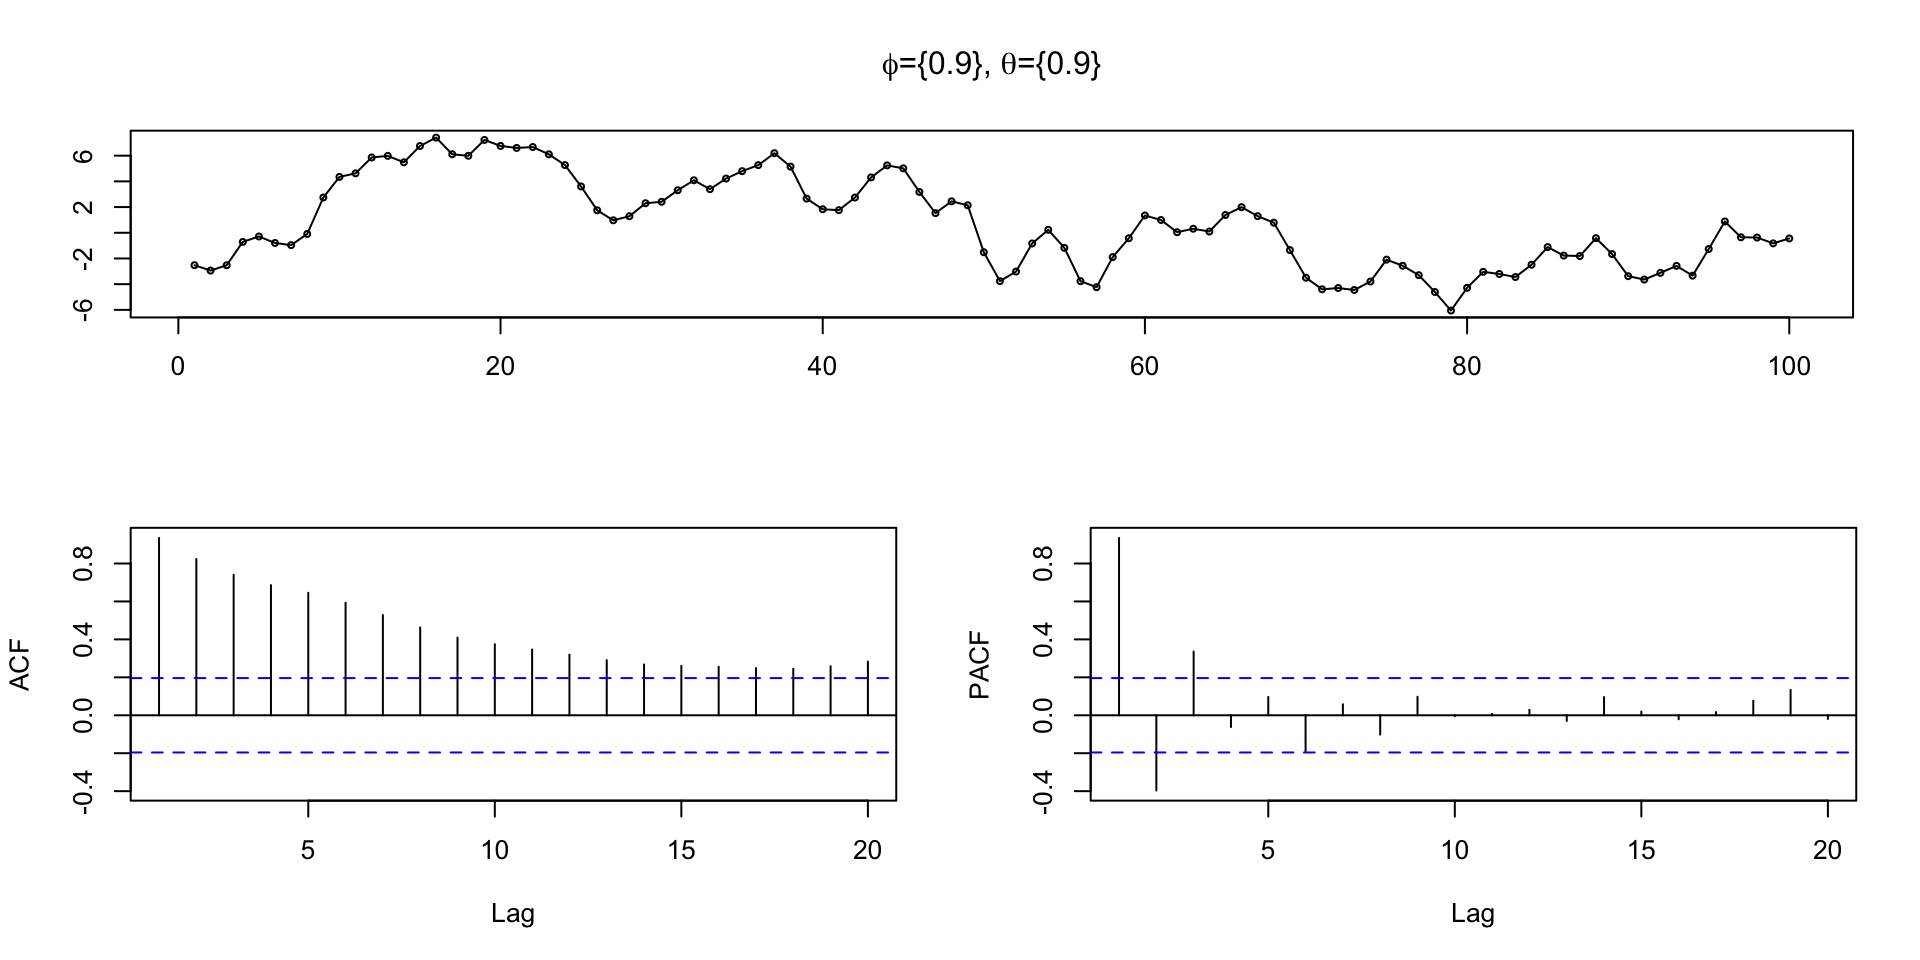
\includegraphics[width=\textwidth]{Lec18_files/figure-beamer/unnamed-chunk-9-1} \end{center}

\end{frame}

\begin{frame}{Residuals}
\protect\hypertarget{residuals}{}

\begin{center}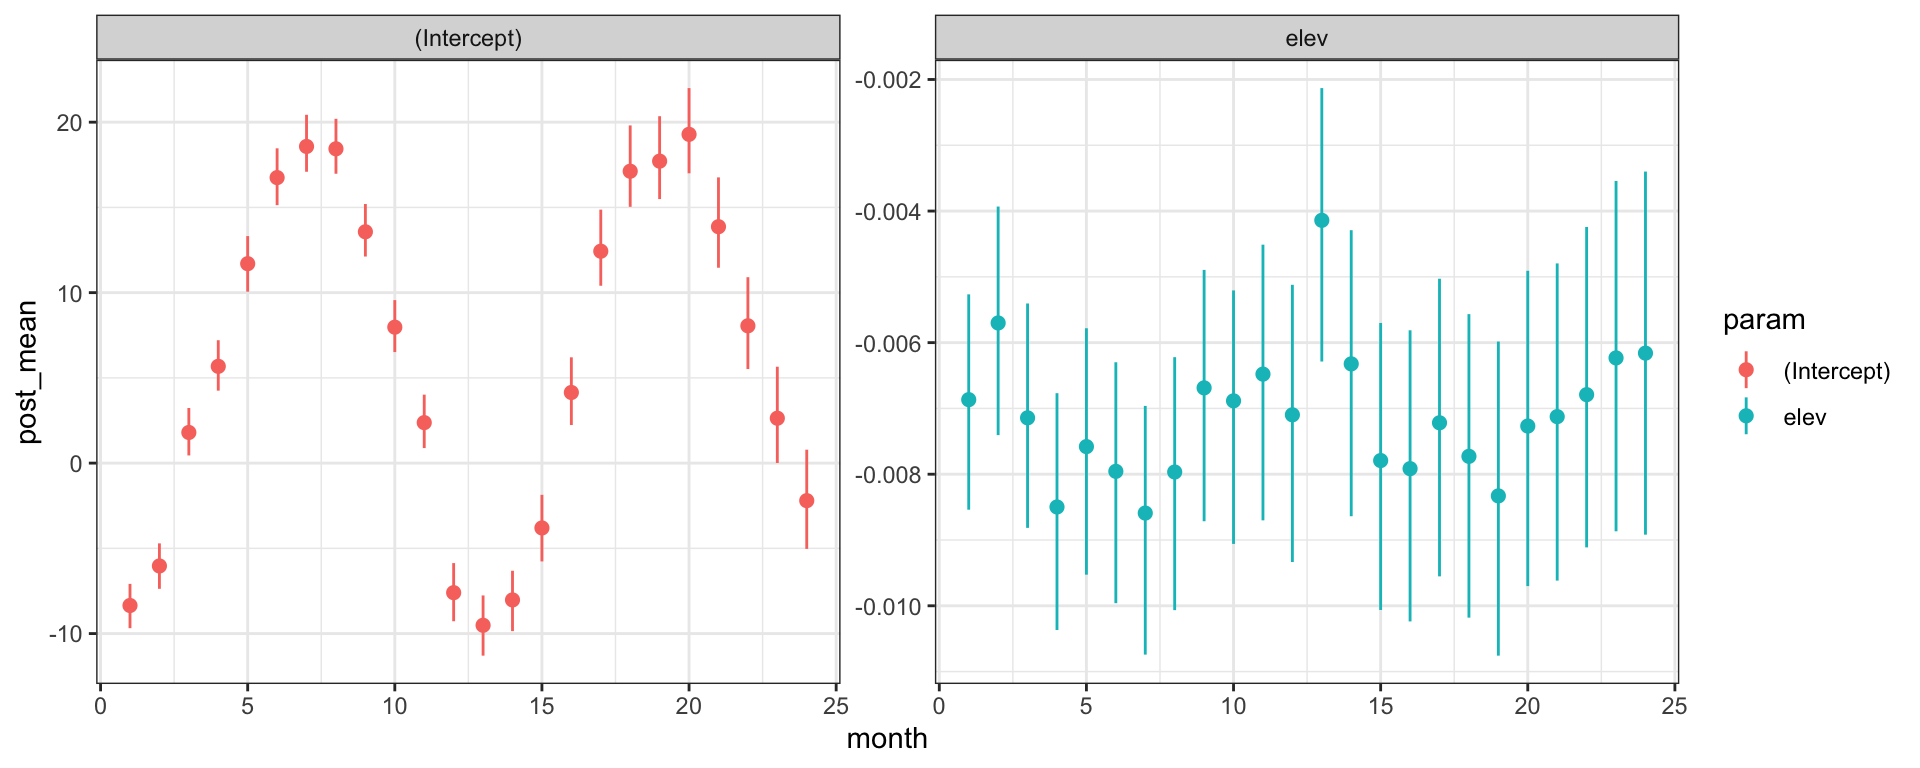
\includegraphics[width=\textwidth]{Lec18_files/figure-beamer/unnamed-chunk-10-1} \end{center}

\end{frame}

\begin{frame}{Predicted vs Observed}
\protect\hypertarget{predicted-vs-observed}{}

\begin{center}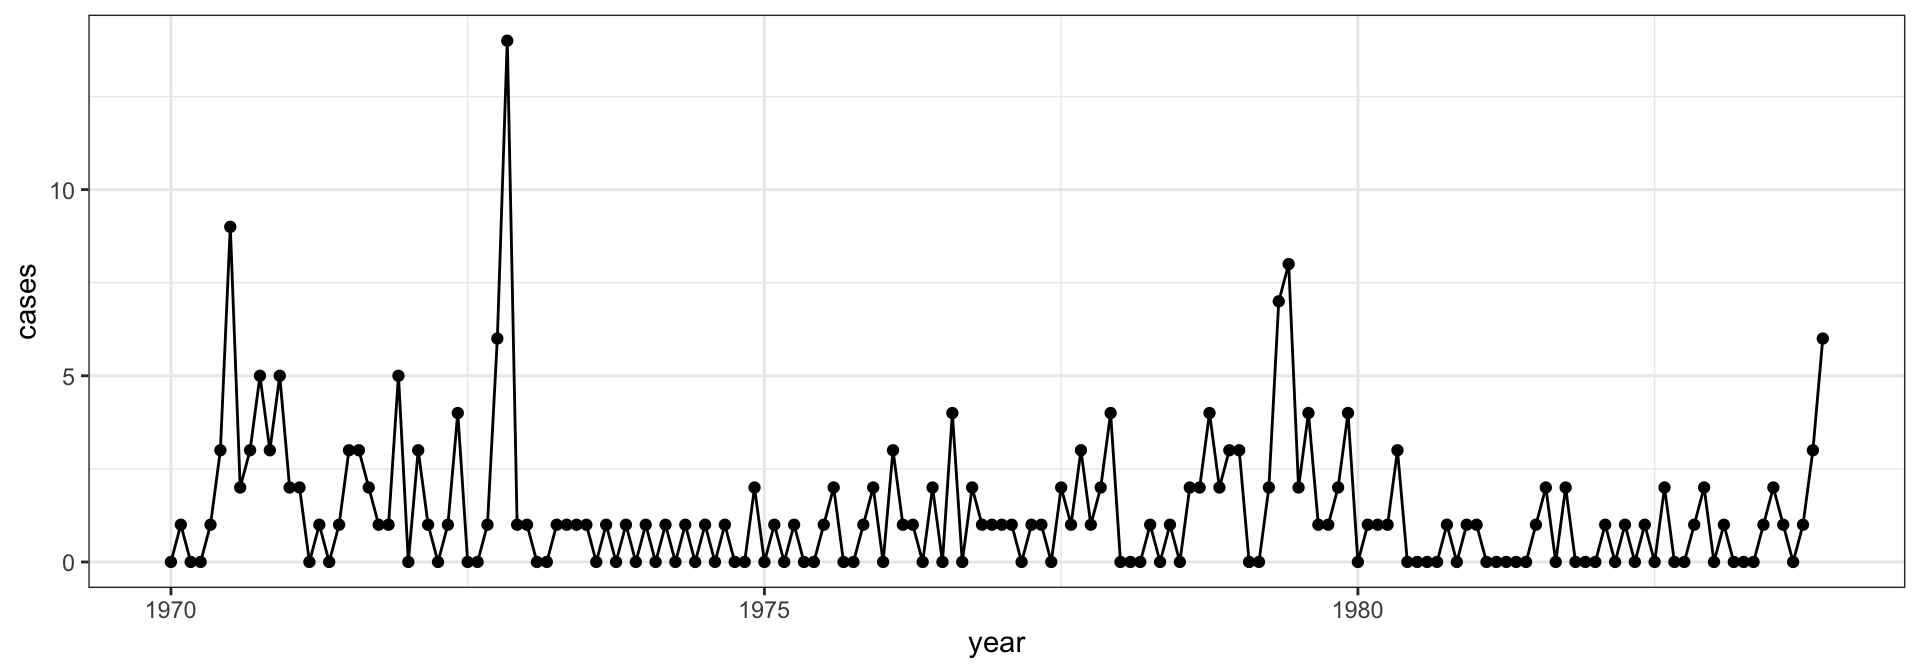
\includegraphics[width=\textwidth]{Lec18_files/figure-beamer/unnamed-chunk-11-1} \end{center}

\end{frame}

\begin{frame}{What's wrong?}
\protect\hypertarget{whats-wrong}{}

\begin{center}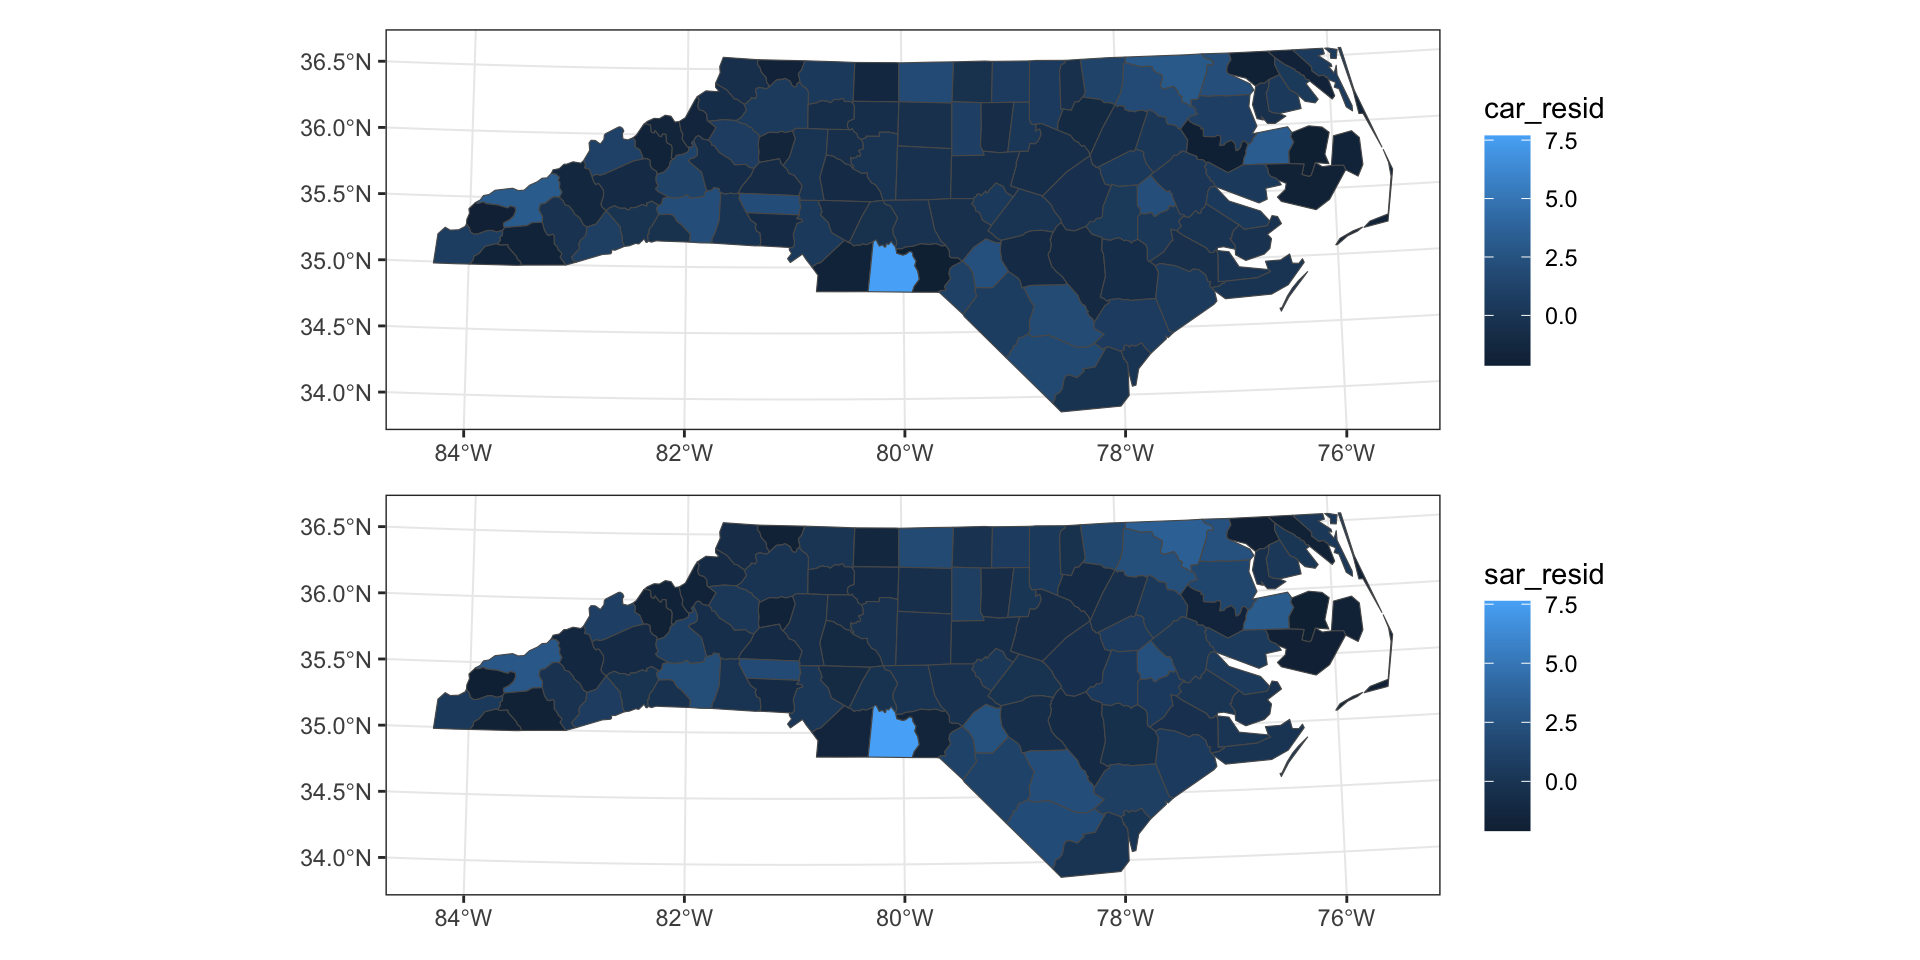
\includegraphics[width=\textwidth]{Lec18_files/figure-beamer/unnamed-chunk-12-1} \end{center}

\end{frame}

\begin{frame}{Comparing CAR vs SAR.}
\protect\hypertarget{comparing-car-vs-sar.}{}

\begin{center}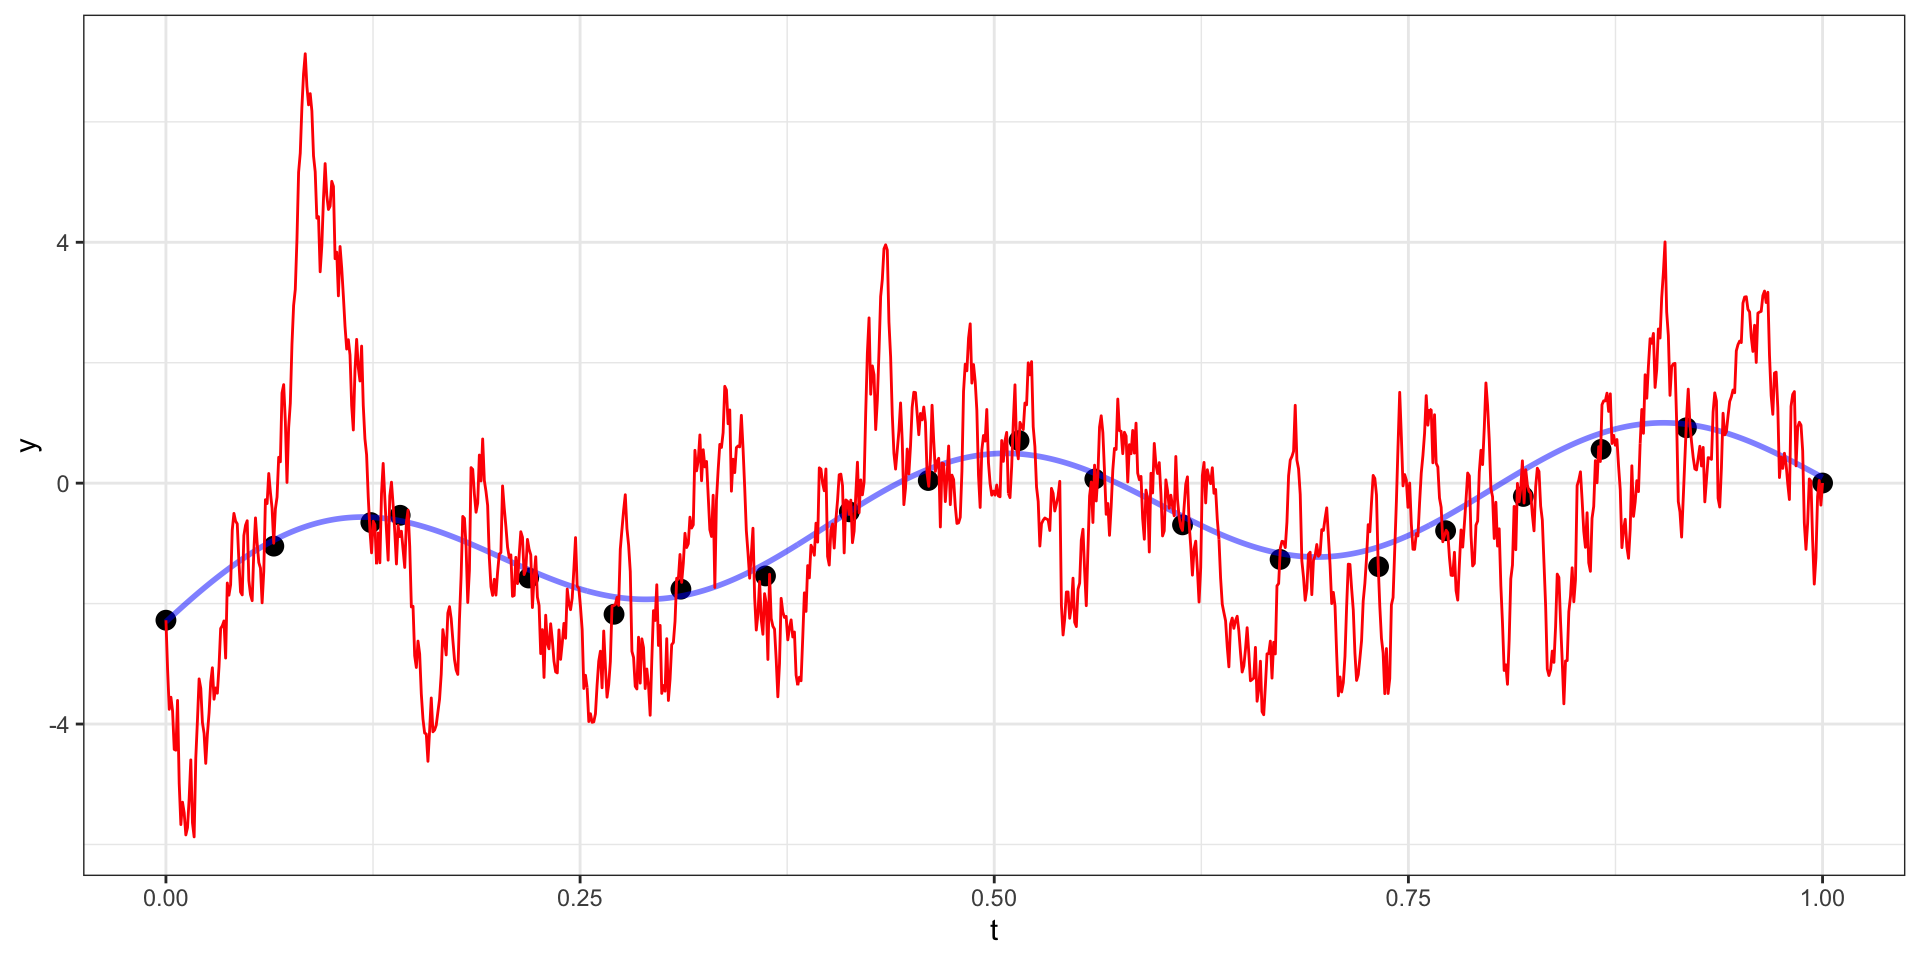
\includegraphics[width=\textwidth]{Lec18_files/figure-beamer/unnamed-chunk-13-1} \end{center}

\end{frame}

\begin{frame}[fragile,t]{Stan CAR Model}
\protect\hypertarget{stan-car-model}{}

\scriptoutput

\begin{Shaded}
\begin{Highlighting}[]
\NormalTok{car_model =}\StringTok{ "}
\StringTok{data \{}
\StringTok{  int<lower=0> N;}
\StringTok{  vector[N] y;}
\StringTok{  matrix[N,N] A;}
\StringTok{  matrix[N,N] D;}
\StringTok{\}}
\StringTok{parameters \{}
\StringTok{  vector[N] w_s;}
\StringTok{  real beta;}
\StringTok{  real<lower=0> sigma2;}
\StringTok{  real<lower=0> sigma2_w;}
\StringTok{  real<lower=0,upper=1> phi;}
\StringTok{\}}
\StringTok{transformed parameters \{}
\StringTok{  vector[N] y_pred = beta + w_s;}
\StringTok{\}}
\StringTok{model \{}
\StringTok{  matrix[N,N] Sigma_inv = (D - phi * A) / sigma2;}
\StringTok{  w_s ~ multi_normal_prec(rep_vector(0,N), Sigma_inv);}

\StringTok{  beta ~ normal(0,10);}
\StringTok{  sigma2 ~ cauchy(0,5);}
\StringTok{  sigma2_w ~ cauchy(0,5);}
\StringTok{  }
\StringTok{  y ~ normal(beta+w_s, sigma2_w);}
\StringTok{\}}
\StringTok{"}
\end{Highlighting}
\end{Shaded}

\end{frame}

\begin{frame}[fragile]{}
\protect\hypertarget{section-2}{}

\begin{Shaded}
\begin{Highlighting}[]
\NormalTok{data =}\StringTok{ }\KeywordTok{list}\NormalTok{(}
  \DataTypeTok{N =} \KeywordTok{nrow}\NormalTok{(nc),}
  \DataTypeTok{y =}\NormalTok{ nc}\OperatorTok{$}\NormalTok{SID74 }\OperatorTok{/}\StringTok{ }\NormalTok{nc}\OperatorTok{$}\NormalTok{BIR74,}
  \DataTypeTok{A =}\NormalTok{ A }\OperatorTok{*}\StringTok{ }\DecValTok{1}\NormalTok{,}
  \DataTypeTok{D =} \KeywordTok{diag}\NormalTok{(}\KeywordTok{rowSums}\NormalTok{(A))}
\NormalTok{)}
\end{Highlighting}
\end{Shaded}

\begin{Shaded}
\begin{Highlighting}[]
\NormalTok{car_fit =}\StringTok{ }\NormalTok{rstan}\OperatorTok{::}\KeywordTok{stan}\NormalTok{(}
  \DataTypeTok{model_code =}\NormalTok{ car_model, }\DataTypeTok{data =}\NormalTok{ data,}
  \DataTypeTok{iter =} \DecValTok{10000}\NormalTok{, }\DataTypeTok{chains =} \DecValTok{1}\NormalTok{, }\DataTypeTok{thin=}\DecValTok{20}
\NormalTok{)}
\end{Highlighting}
\end{Shaded}

\pause

\vspace{10mm}

Why don't we use the conditional definition for the \(y\)'s?

\end{frame}

\begin{frame}{Model Results}
\protect\hypertarget{model-results}{}

\begin{center}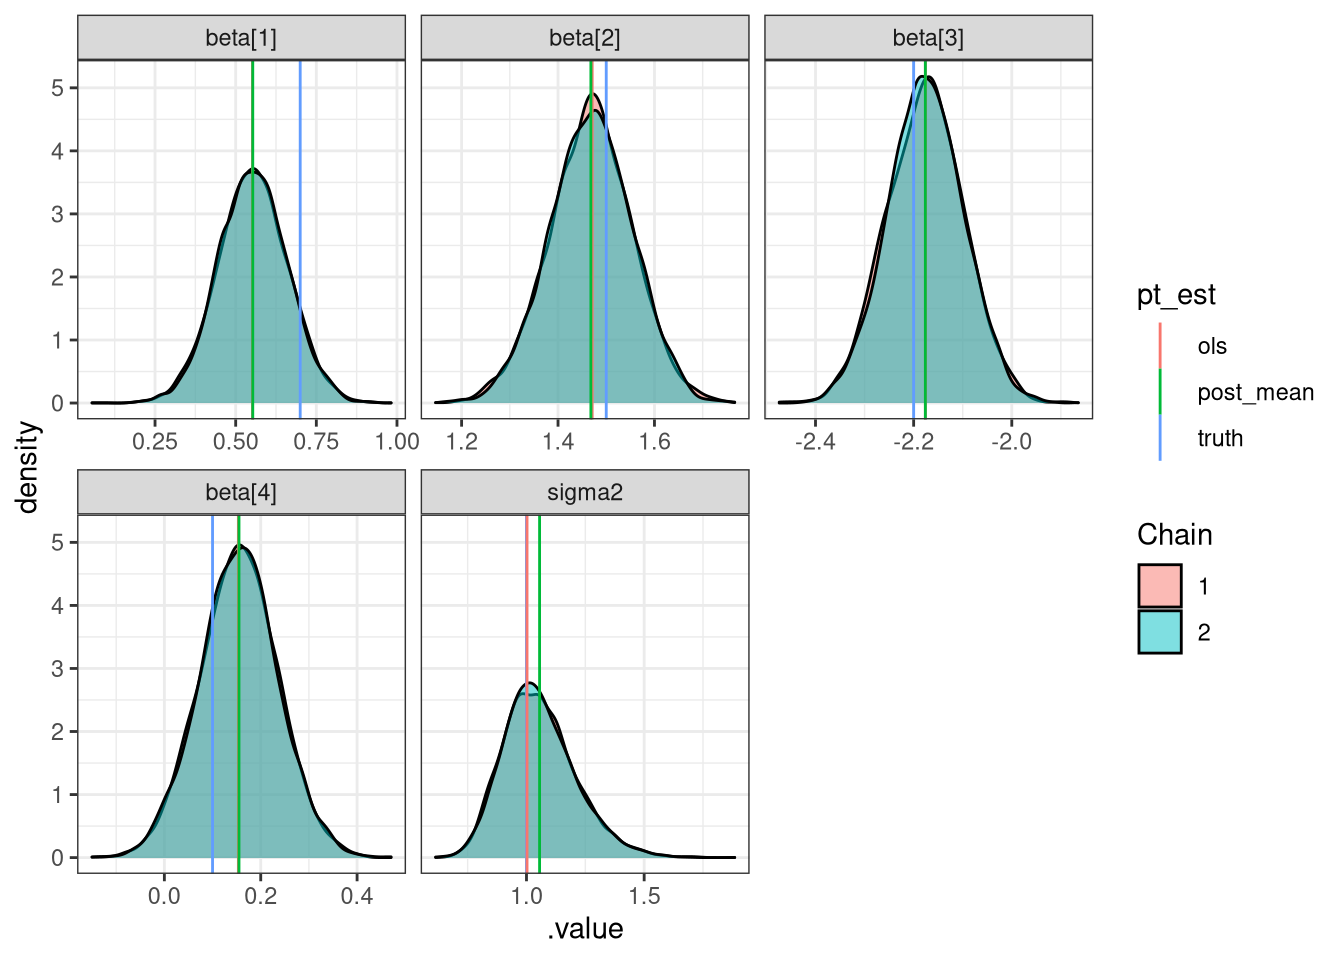
\includegraphics[width=\textwidth]{Lec18_files/figure-beamer/unnamed-chunk-19-1} \end{center}

\end{frame}

\begin{frame}{Predictions}
\protect\hypertarget{predictions-1}{}

\begin{center}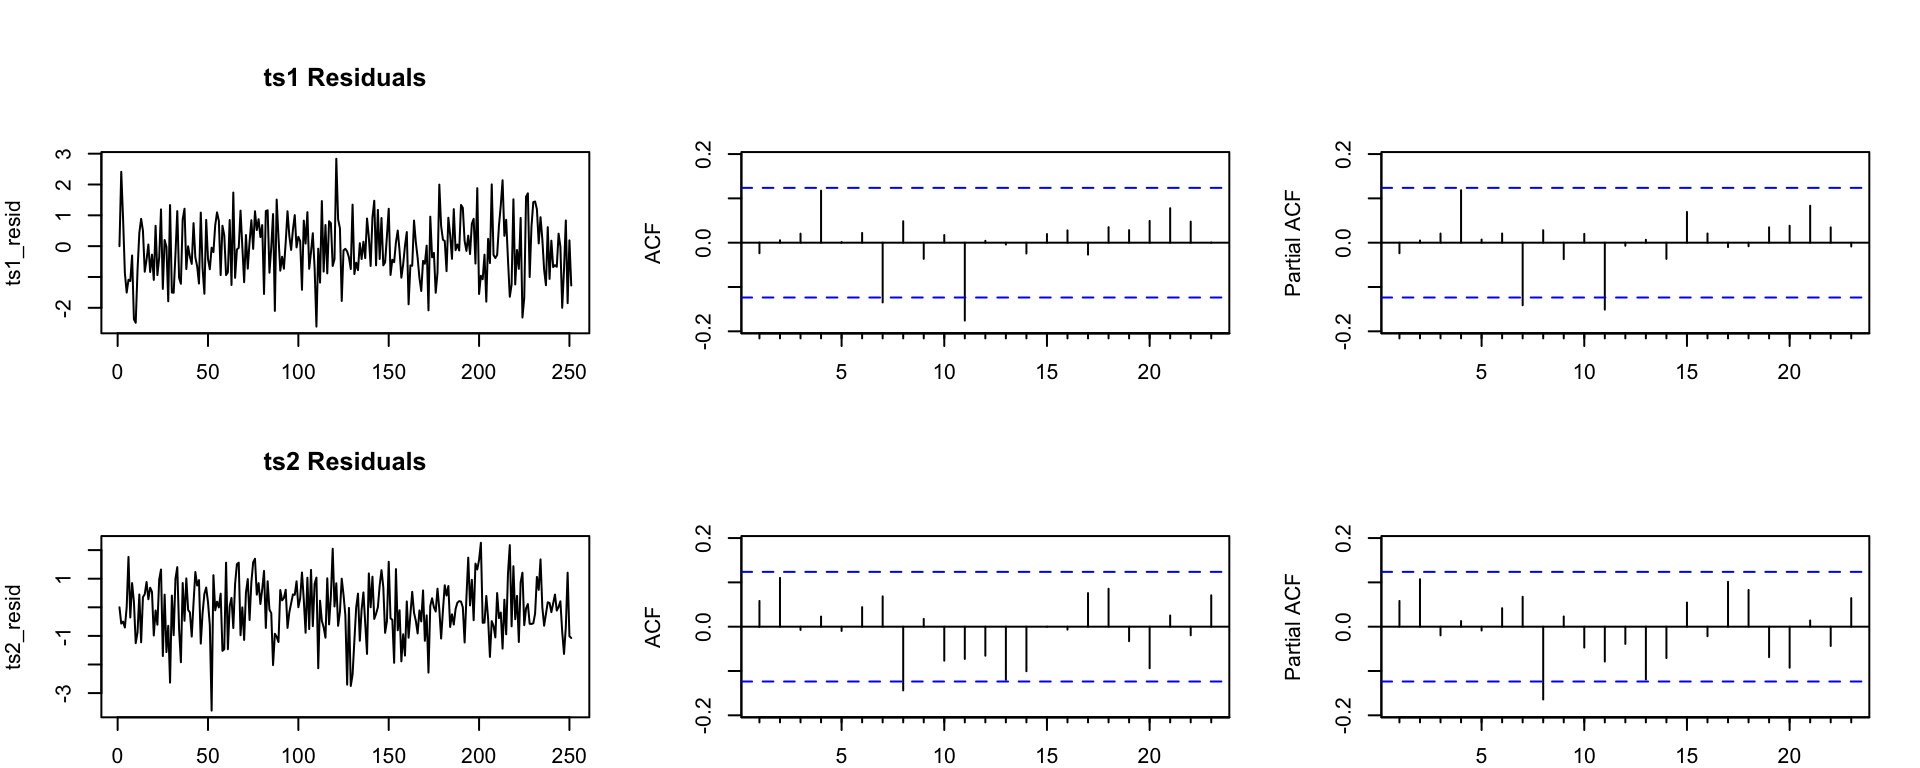
\includegraphics[width=\textwidth]{Lec18_files/figure-beamer/unnamed-chunk-21-1} \end{center}

\end{frame}

\begin{frame}{}
\protect\hypertarget{section-3}{}

\begin{center}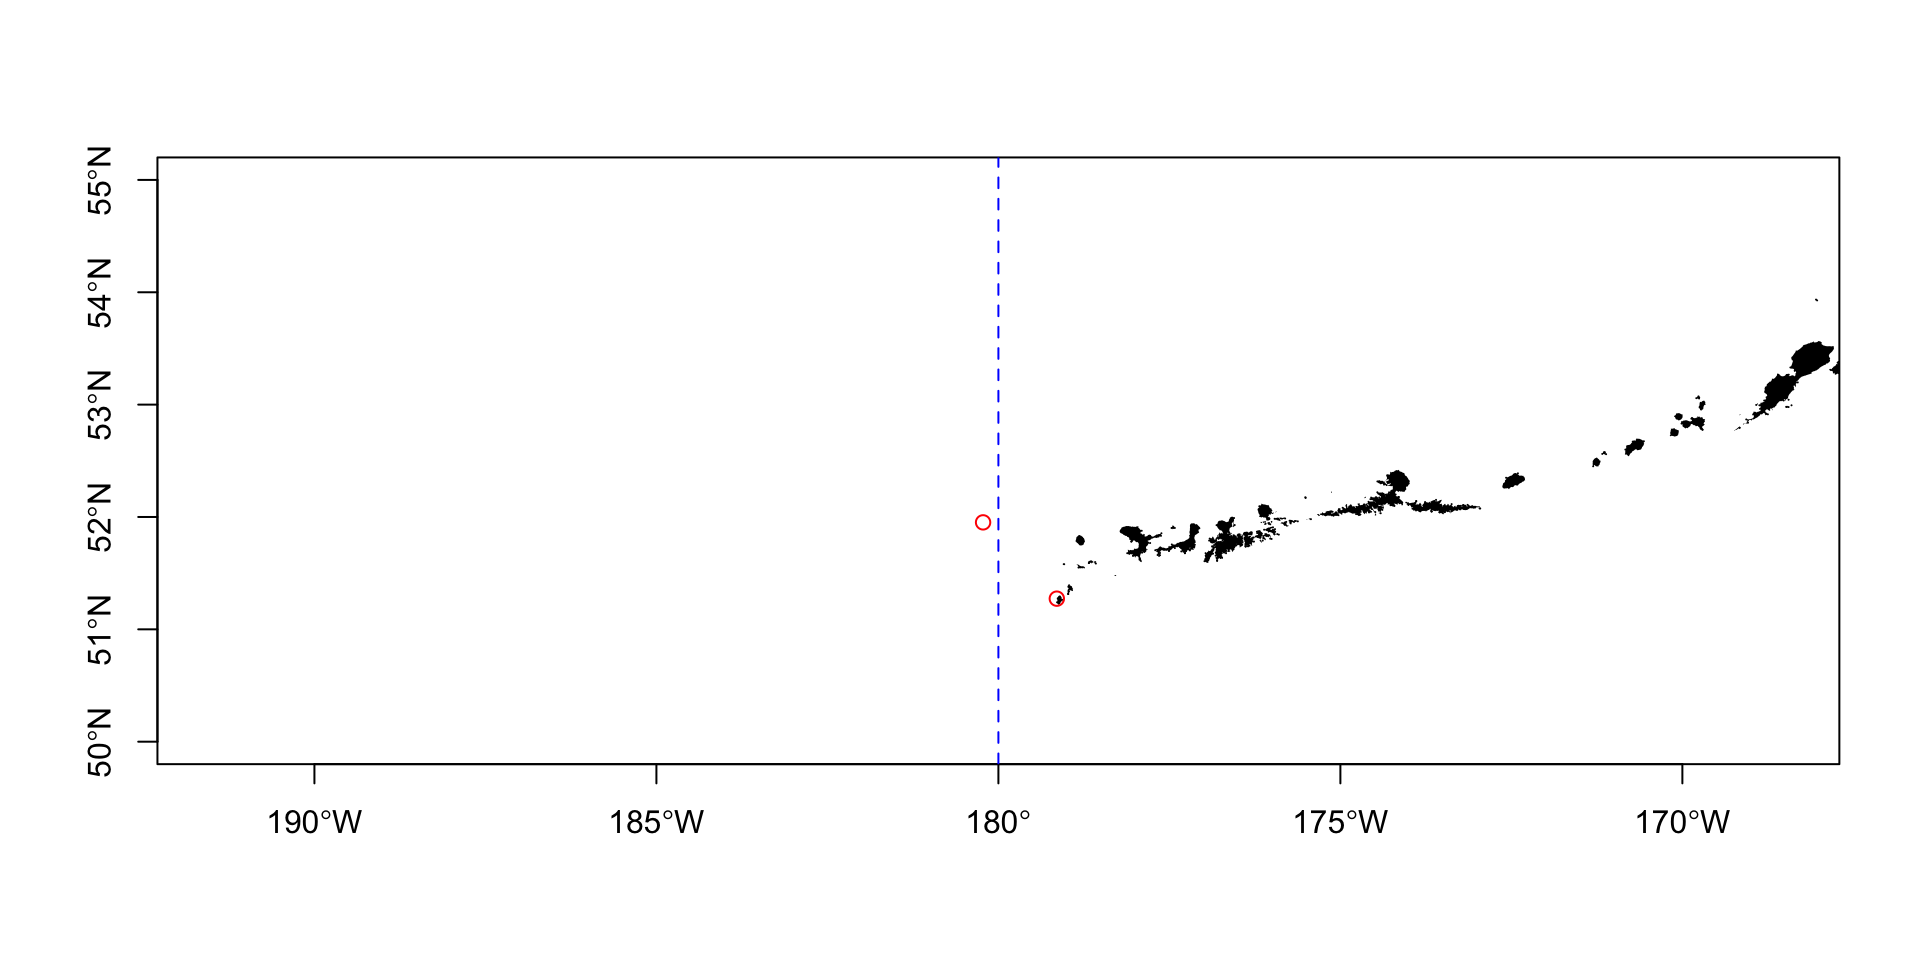
\includegraphics[width=\textwidth]{Lec18_files/figure-beamer/unnamed-chunk-22-1} \end{center}

\end{frame}

\begin{frame}{Brief Aside - SAR Precision Matrix}
\protect\hypertarget{brief-aside---sar-precision-matrix}{}

\[ 
\Sigma_{SAR} = (\symbf{I}-\phi \symbf{D}^{-1} \, \symbf{A})^{-1} \sigma^2 \, \symbf{D}^{-1} \left((\symbf{I}-\phi \symbf{D}^{-1} \, \symbf{A})^{-1}\right)^t
\]

\vspace{6mm}

\[ \begin{aligned}
\Sigma^{-1}_{SAR} 
  &= \left( (\symbf{I}-\phi \symbf{D}^{-1} \, \symbf{A})^{-1} \sigma^2 \, \symbf{D}^{-1} \left((\symbf{I}-\phi \symbf{D}^{-1} \, \symbf{A})^{-1}\right)^t \right)^{-1} \\
  &= \left( \left( (\symbf{I}-\phi \symbf{D}^{-1} \, \symbf{A})^{-1}\right)^t\right)^{-1} \frac{1}{\sigma^2} \, \symbf{D} ~ (\symbf{I}-\phi \symbf{D}^{-1} \, \symbf{A}) \\
  &= \frac{1}{\sigma^2} \, (\symbf{I}-\phi \symbf{D}^{-1} \, \symbf{A})^t ~ \symbf{D} ~ (\symbf{I}-\phi \symbf{D}^{-1} \, \symbf{A}) \\
\end{aligned}\]

\end{frame}

\begin{frame}[fragile,t]{Jags SAR Model}
\protect\hypertarget{jags-sar-model}{}

\tinyoutput

\begincols

\begincol{0.5\textwidth}

\begin{Shaded}
\begin{Highlighting}[]
\NormalTok{sar_model =}\StringTok{ "}
\StringTok{data \{}
\StringTok{  int<lower=0> N;}
\StringTok{  vector[N] y;}
\StringTok{  matrix[N,N] W_tilde;}
\StringTok{  matrix[N,N] D;}
\StringTok{\}}
\StringTok{transformed data \{}
\StringTok{  matrix[N,N] I = diag_matrix(rep_vector(1, N));}
\StringTok{\}}
\StringTok{parameters \{}
\StringTok{  vector[N] w_s;}
\StringTok{  real beta;}
\StringTok{  real<lower=0> sigma2;}
\StringTok{  real<lower=0> sigma2_w;}
\StringTok{  real<lower=0,upper=1> phi;}
\StringTok{\}}
\StringTok{transformed parameters \{}
\StringTok{  vector[N] y_pred = beta + w_s;}
\StringTok{\}}
\StringTok{model \{}
\StringTok{  matrix[N,N] C = I - phi * W_tilde;}
\StringTok{  matrix[N,N] Sigma_inv = C' * D * C / sigma2;  }
\StringTok{  }
\StringTok{  w_s ~ multi_normal_prec(rep_vector(0,N), Sigma_inv);}

\StringTok{  beta ~ normal(0,10);}
\StringTok{  sigma2 ~ cauchy(0,5);}
\StringTok{  sigma2_w ~ cauchy(0,5);}

\StringTok{  y ~ normal(beta + w_s, sigma2_w);}
\StringTok{\}}
\StringTok{"}
\end{Highlighting}
\end{Shaded}

\endcol

\begincol{0.5\textwidth}

\begin{Shaded}
\begin{Highlighting}[]
\NormalTok{D =}\StringTok{ }\KeywordTok{diag}\NormalTok{(}\KeywordTok{rowSums}\NormalTok{(A))}
\NormalTok{D_inv =}\StringTok{ }\KeywordTok{diag}\NormalTok{(}\DecValTok{1}\OperatorTok{/}\KeywordTok{diag}\NormalTok{(D))}
\NormalTok{data =}\StringTok{ }\KeywordTok{list}\NormalTok{(}
  \DataTypeTok{N =} \KeywordTok{nrow}\NormalTok{(nc),}
  \DataTypeTok{y =}\NormalTok{ nc}\OperatorTok{$}\NormalTok{SID74 }\OperatorTok{/}\StringTok{ }\NormalTok{nc}\OperatorTok{$}\NormalTok{BIR74,}
  \DataTypeTok{x =} \KeywordTok{rep}\NormalTok{(}\DecValTok{1}\NormalTok{, }\KeywordTok{nrow}\NormalTok{(nc)),}
  \DataTypeTok{D_inv =}\NormalTok{ D_inv,}
  \DataTypeTok{W_tilde =}\NormalTok{ D_inv }\OperatorTok\StringTok{ }\NormalTok{A}
\NormalTok{)}
\end{Highlighting}
\end{Shaded}

\begin{Shaded}
\begin{Highlighting}[]
\NormalTok{sar_fit =}\StringTok{ }\NormalTok{rstan}\OperatorTok{::}\KeywordTok{stan}\NormalTok{(}
  \DataTypeTok{model_code =}\NormalTok{ sar_model, }\DataTypeTok{data =}\NormalTok{ data,}
  \DataTypeTok{iter =} \DecValTok{10000}\NormalTok{, }\DataTypeTok{chains =} \DecValTok{1}\NormalTok{, }\DataTypeTok{thin=}\DecValTok{20}
\NormalTok{)}
\end{Highlighting}
\end{Shaded}

\endcol

\endcols

\end{frame}

\begin{frame}{Model Results}
\protect\hypertarget{model-results-1}{}

\begin{center}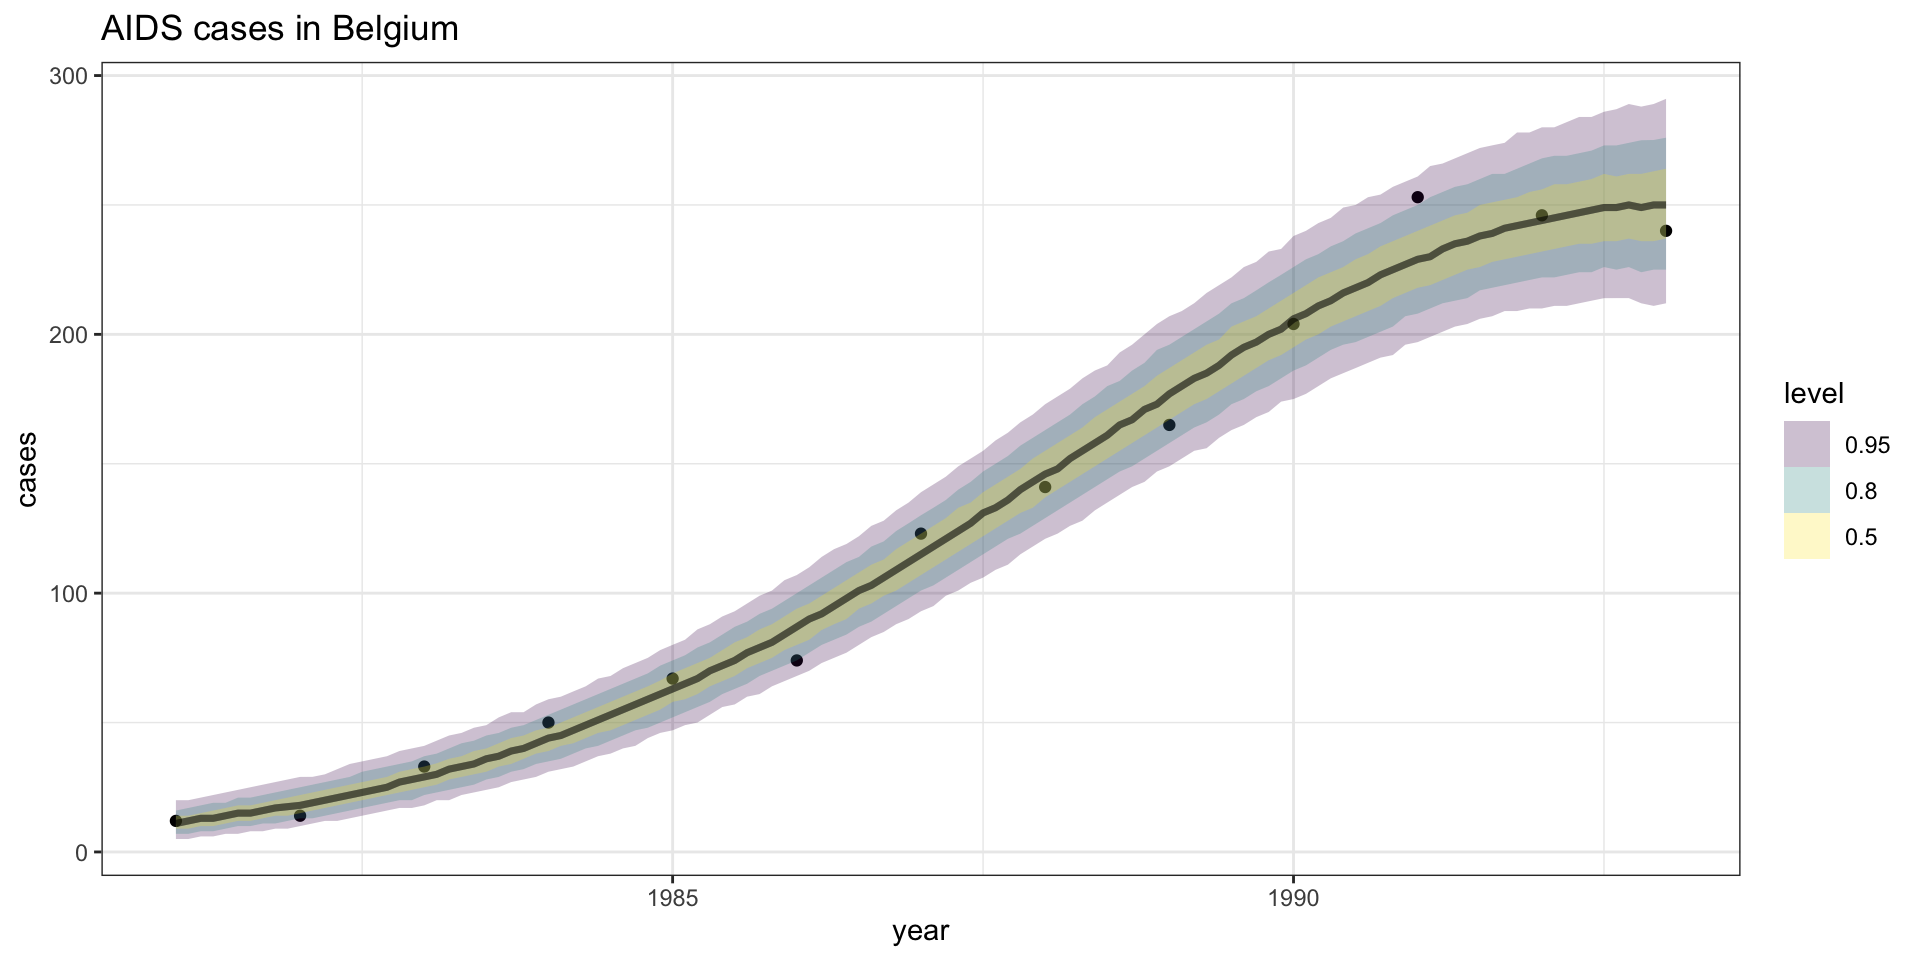
\includegraphics[width=\textwidth]{Lec18_files/figure-beamer/unnamed-chunk-28-1} \end{center}

\end{frame}

\begin{frame}[t]{Predictions}
\protect\hypertarget{predictions-2}{}

\begin{center}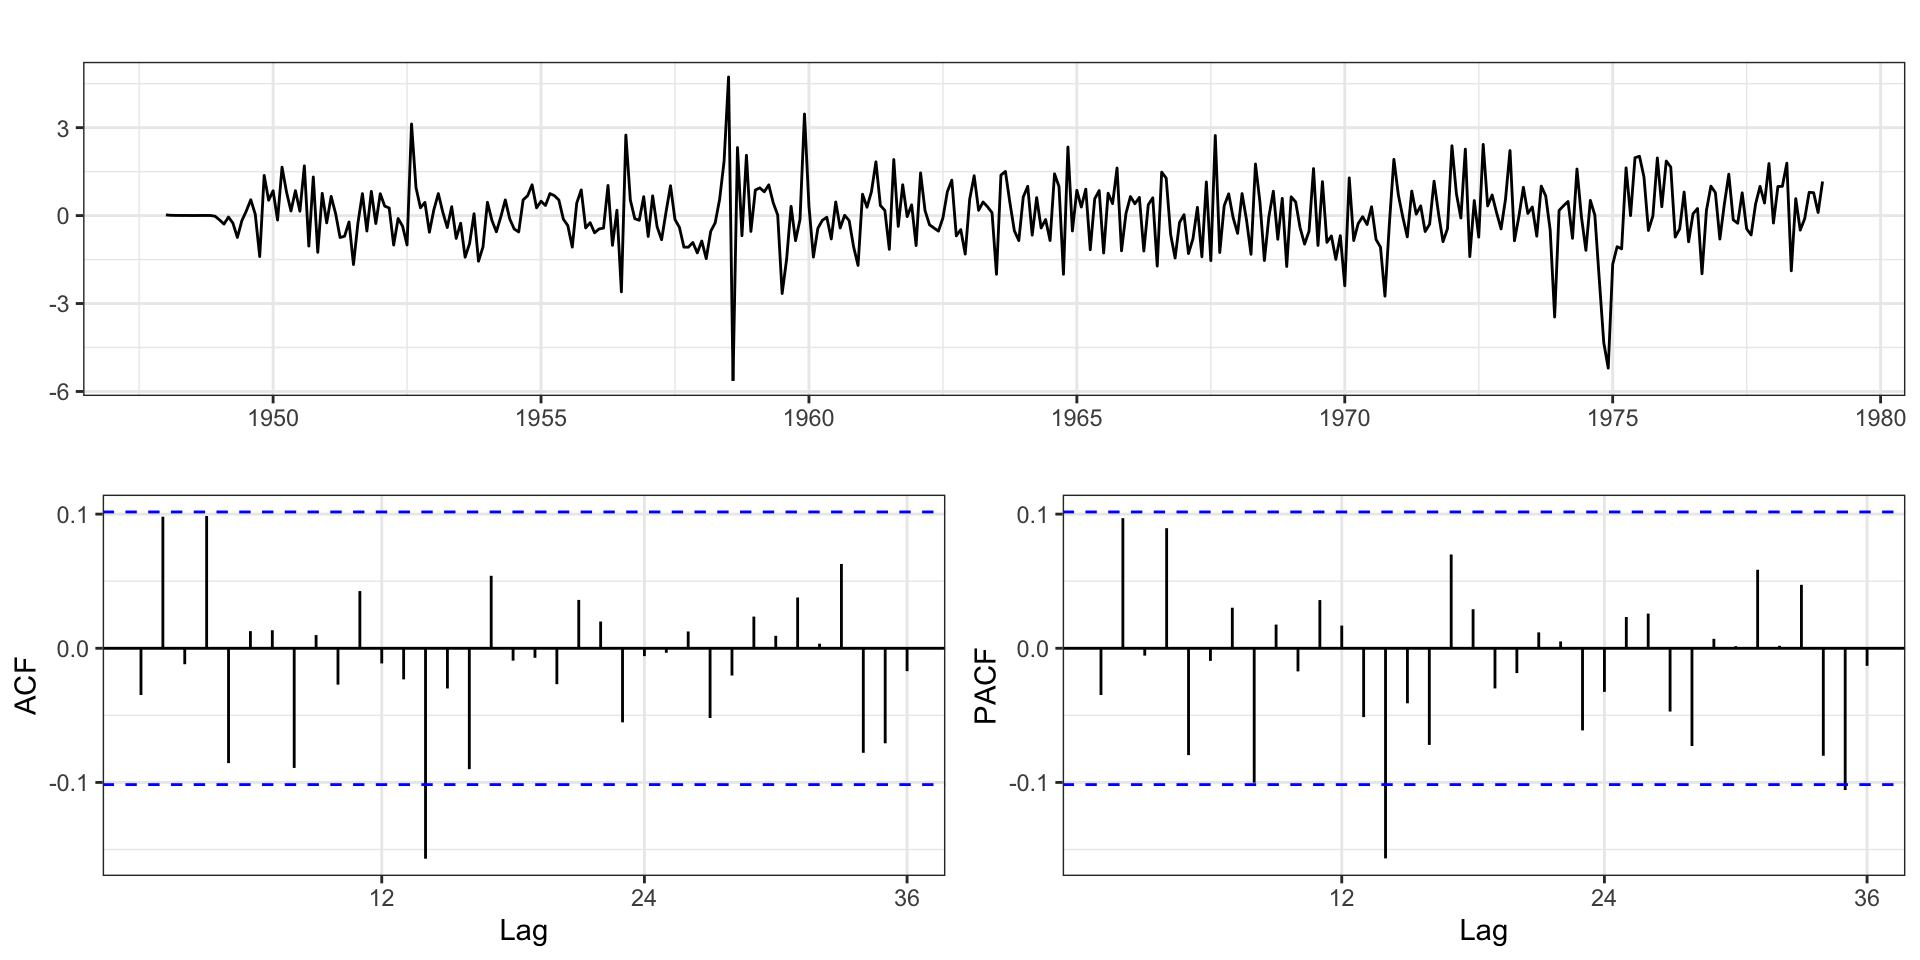
\includegraphics[width=\textwidth]{Lec18_files/figure-beamer/unnamed-chunk-30-1} \end{center}

\end{frame}

\begin{frame}{}
\protect\hypertarget{section-4}{}

\begin{center}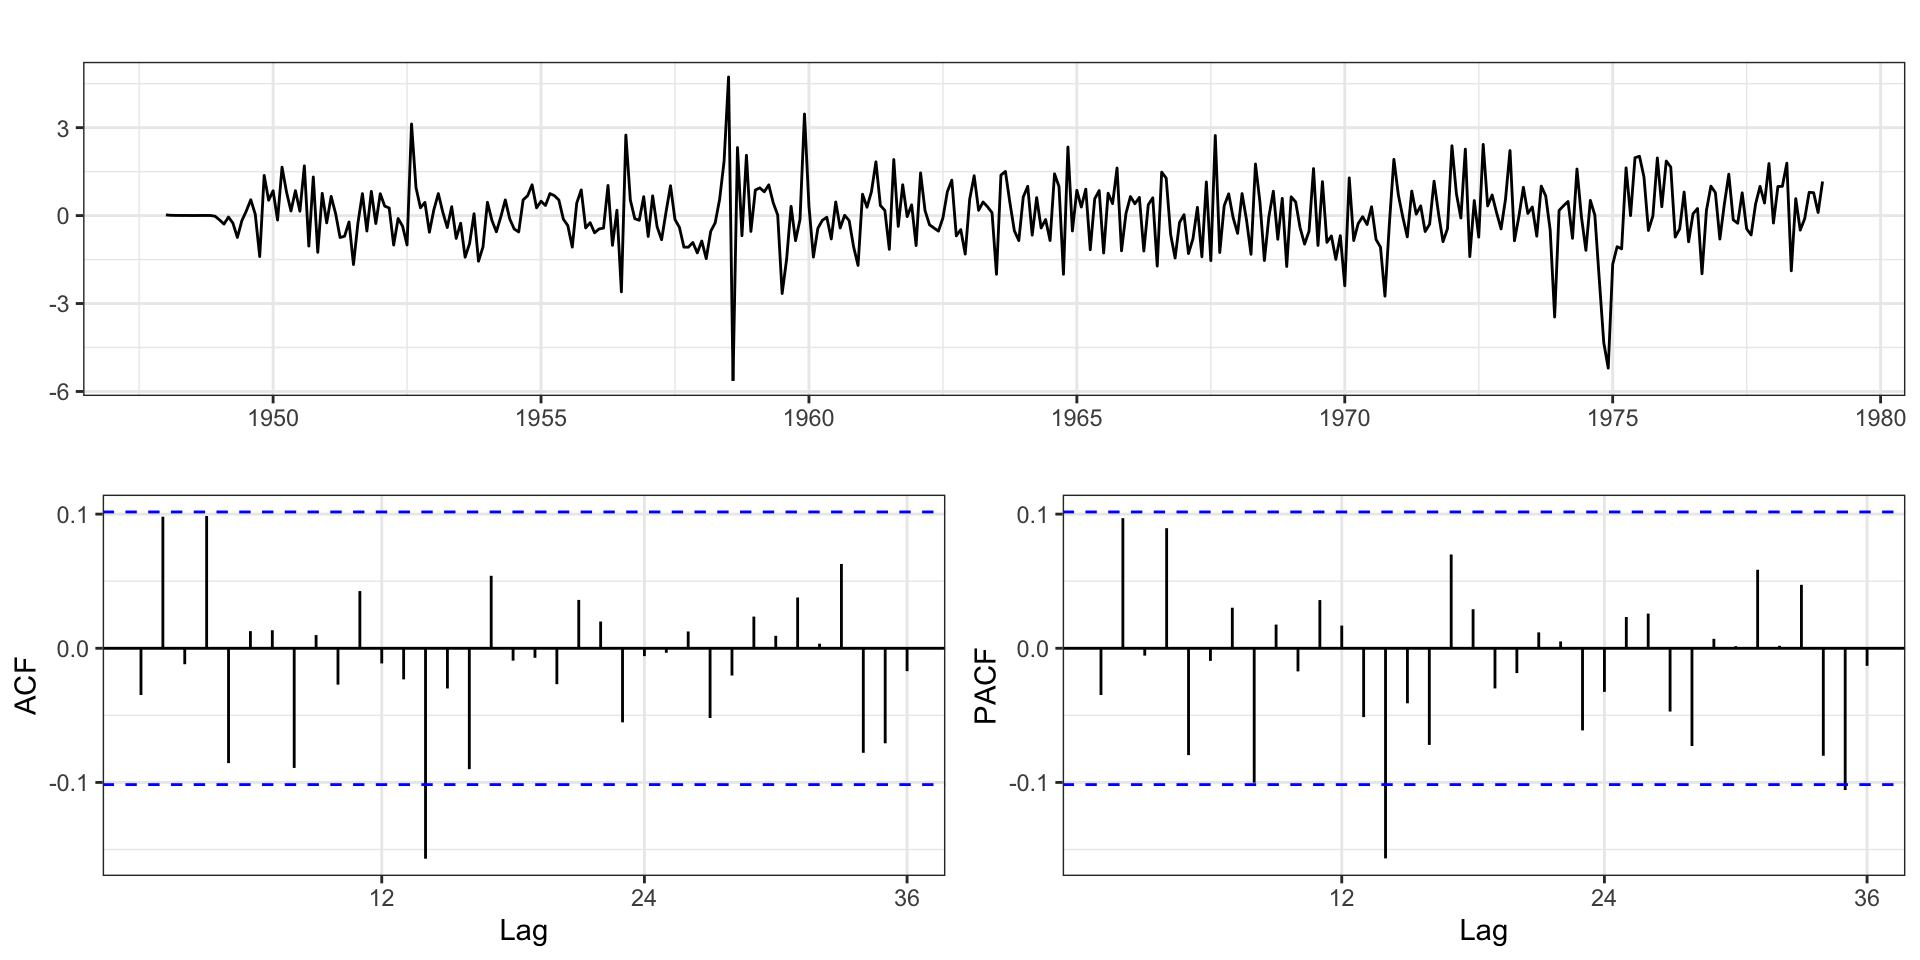
\includegraphics[width=\textwidth]{Lec18_files/figure-beamer/unnamed-chunk-31-1} \end{center}

\end{frame}

\begin{frame}[fragile,t]{Comparing Predictions}
\protect\hypertarget{comparing-predictions}{}

\begin{Shaded}
\begin{Highlighting}[]
\CommentTok{# RMSE}
\KeywordTok{sqrt}\NormalTok{(}\KeywordTok{mean}\NormalTok{(nc}\OperatorTok{$}\NormalTok{bayes_car_resid}\OperatorTok{^}\DecValTok{2}\NormalTok{))}
\CommentTok{## [1] 0.0002092447}

\KeywordTok{sqrt}\NormalTok{(}\KeywordTok{mean}\NormalTok{(nc}\OperatorTok{$}\NormalTok{bayes_sar_resid}\OperatorTok{^}\DecValTok{2}\NormalTok{))}
\CommentTok{## [1] 0.0002983034}

\KeywordTok{sqrt}\NormalTok{(}\KeywordTok{mean}\NormalTok{(nc}\OperatorTok{$}\NormalTok{car_resid}\OperatorTok{^}\DecValTok{2}\NormalTok{))}
\CommentTok{## [1] 0.001448564}

\KeywordTok{sqrt}\NormalTok{(}\KeywordTok{mean}\NormalTok{(nc}\OperatorTok{$}\NormalTok{sar_resid}\OperatorTok{^}\DecValTok{2}\NormalTok{))}
\CommentTok{## [1] 0.001470432}
\end{Highlighting}
\end{Shaded}

\end{frame}

\begin{frame}{Comparing Parameters}
\protect\hypertarget{comparing-parameters}{}

\begin{center}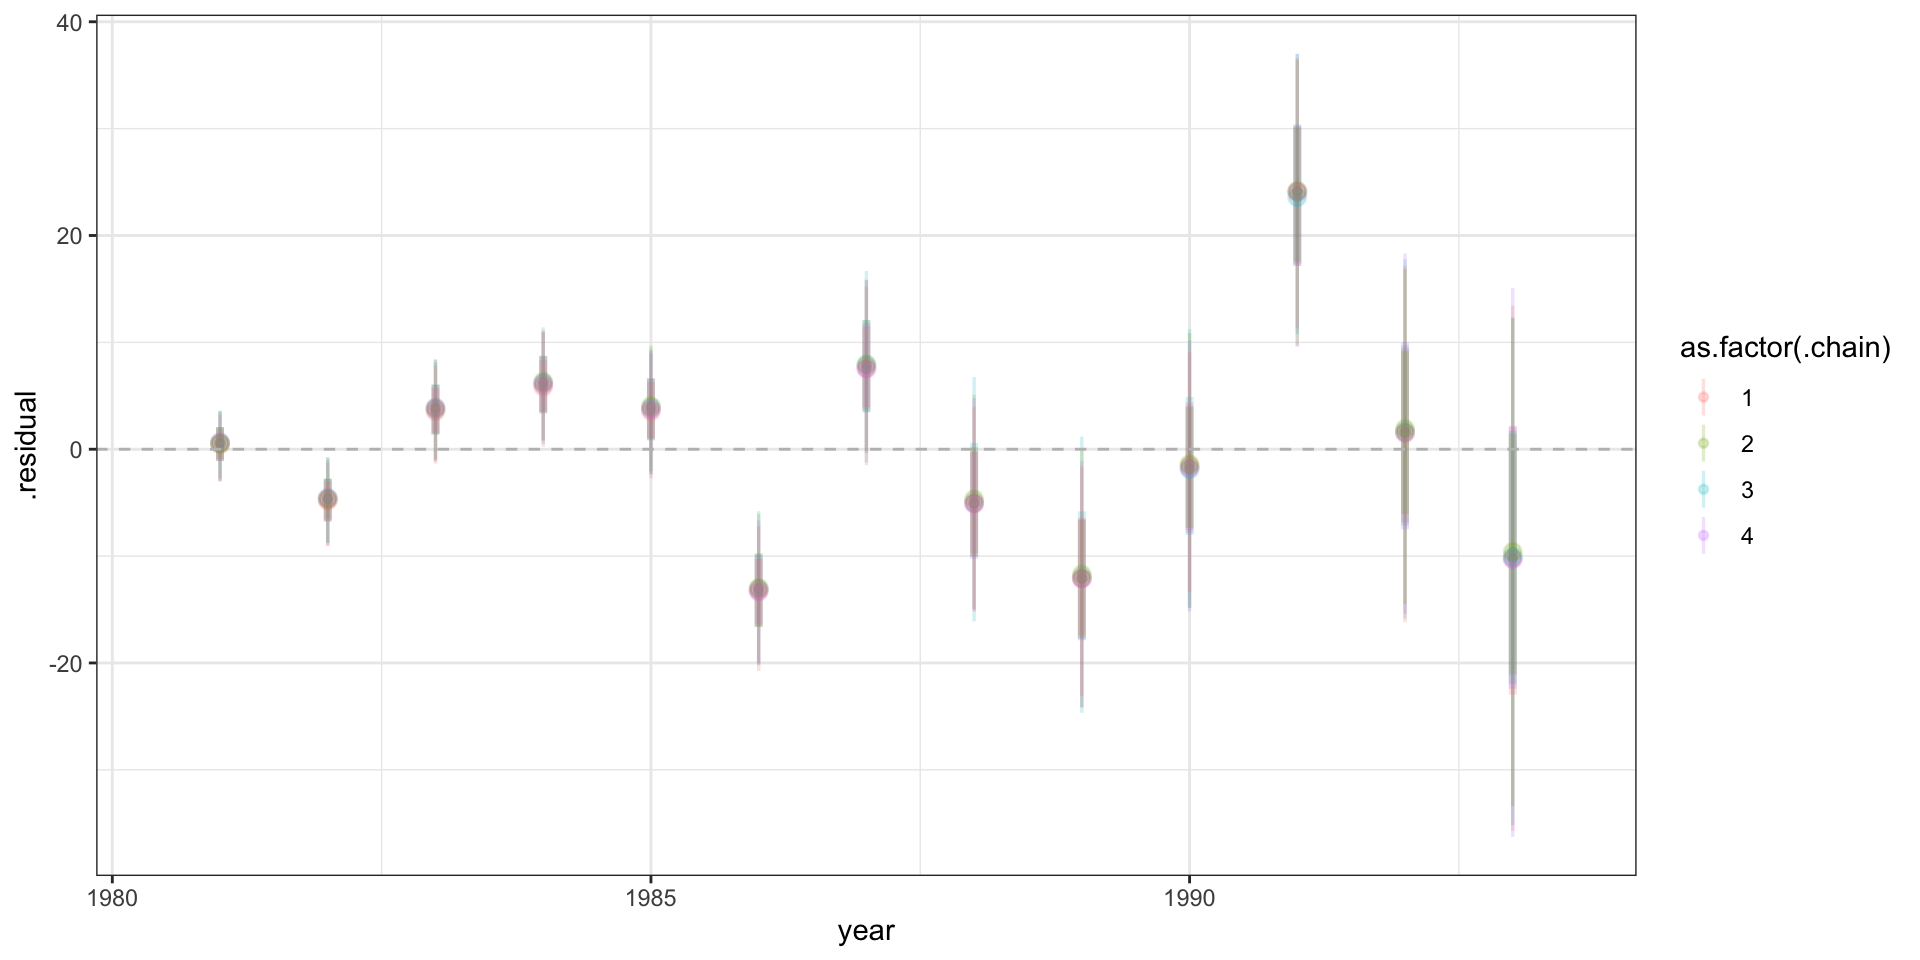
\includegraphics[width=\textwidth]{Lec18_files/figure-beamer/unnamed-chunk-33-1} \end{center}

\end{frame}

\begin{frame}{CAR vs SAR?}
\protect\hypertarget{car-vs-sar}{}

\end{frame}

\hypertarget{transforming-the-data}{%
\section{Transforming the data}\label{transforming-the-data}}

\begin{frame}{Freeman-Tukey's transformation}
\protect\hypertarget{freeman-tukeys-transformation}{}

This is the transformation used by Cressie and Road in Spatial Data
Analysis of Regional Counts (1989).

\footnotesize

\[
FT = \sqrt{1000} \left( \sqrt{\frac{SID74}{BIR74}} + \sqrt{\frac{SID74+1}{BIR74}} \right)
\]

\begin{center}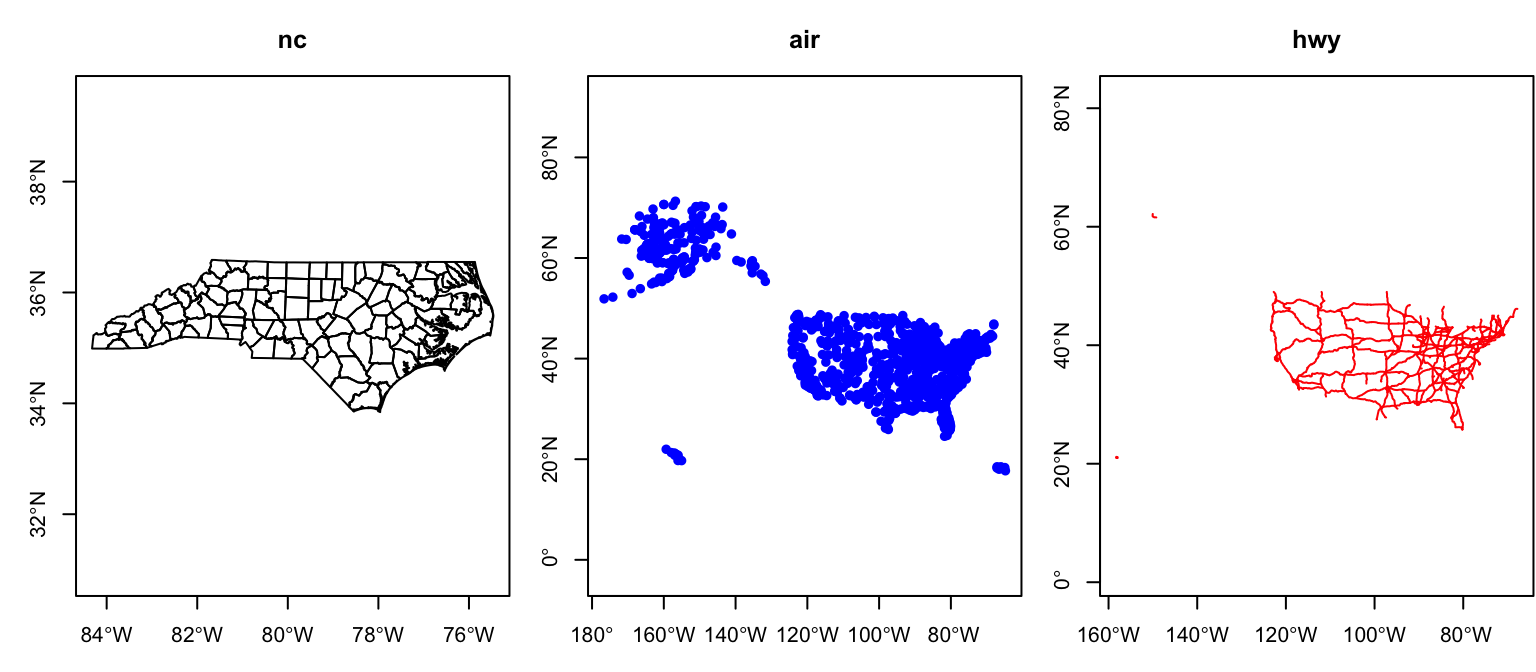
\includegraphics[width=\textwidth]{Lec18_files/figure-beamer/unnamed-chunk-34-1} \end{center}

\end{frame}

\begin{frame}[fragile]{Other options}
\protect\hypertarget{other-options}{}

\scriptoutput

\begin{Shaded}
\begin{Highlighting}[]
\NormalTok{nc =}\StringTok{ }\KeywordTok{mutate}\NormalTok{(nc, }
  \DataTypeTok{sqrt =} \KeywordTok{sqrt}\NormalTok{((SID74}\OperatorTok{+}\DecValTok{1}\NormalTok{)}\OperatorTok{/}\NormalTok{BIR74),}
  \DataTypeTok{log  =} \KeywordTok{log}\NormalTok{((SID74}\OperatorTok{+}\DecValTok{1}\NormalTok{)}\OperatorTok{/}\NormalTok{BIR74),}
\NormalTok{)}
\end{Highlighting}
\end{Shaded}

\begin{center}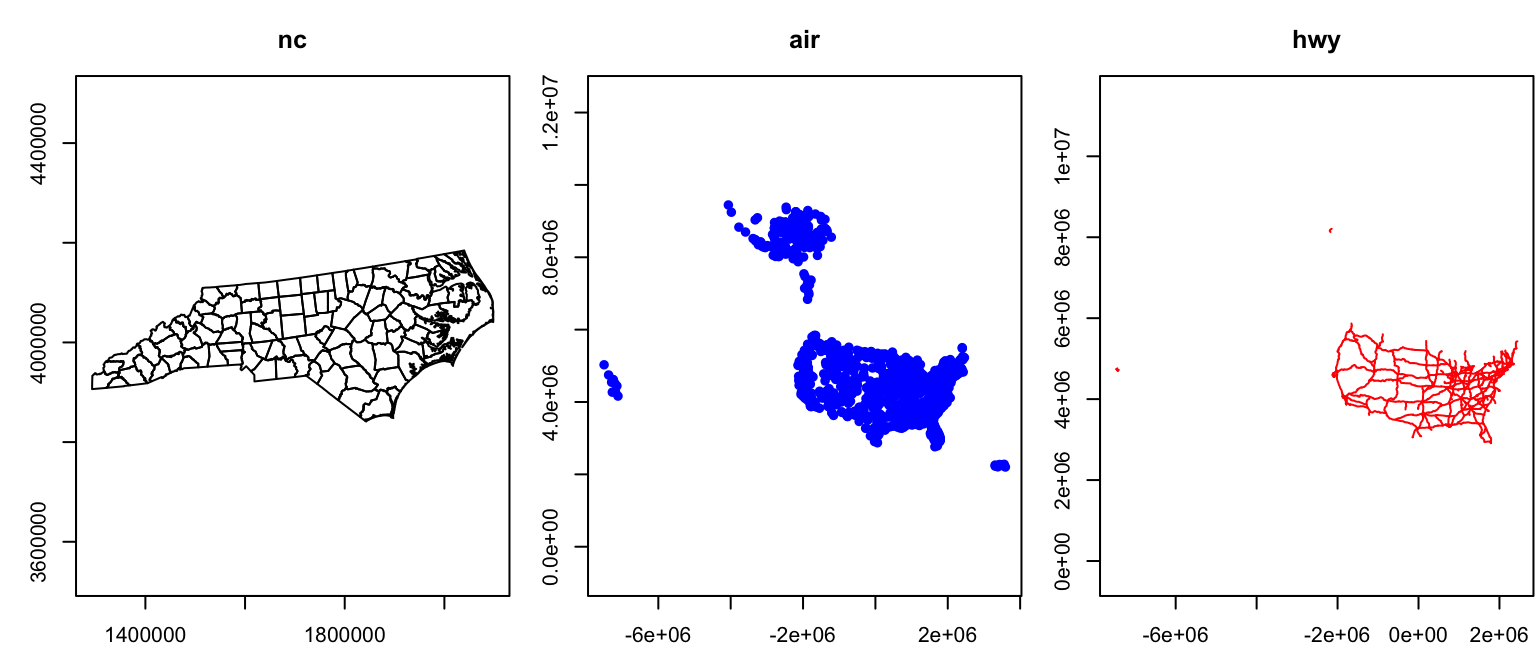
\includegraphics[width=\textwidth]{Lec18_files/figure-beamer/unnamed-chunk-36-1} \end{center}

\end{frame}

\begin{frame}[fragile]{log transformation}
\protect\hypertarget{log-transformation}{}

\scriptoutput

\begin{center}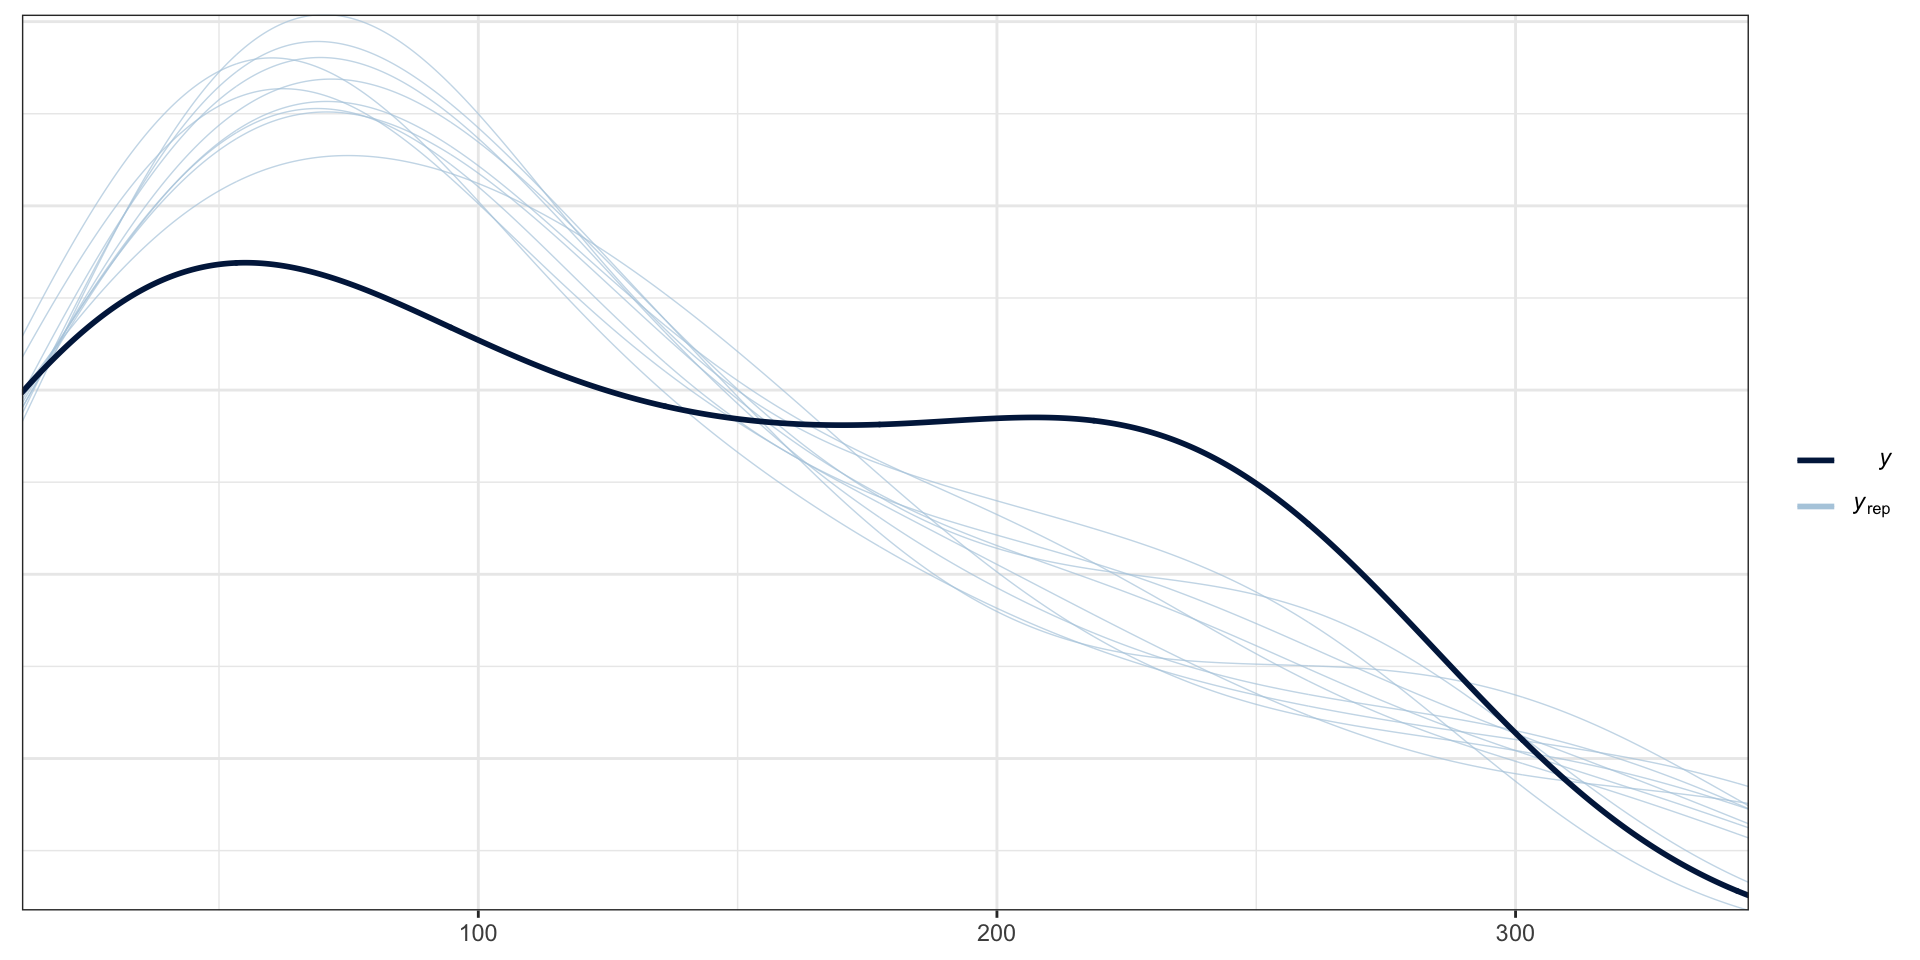
\includegraphics[width=\textwidth]{Lec18_files/figure-beamer/unnamed-chunk-37-1} \end{center}

\begin{verbatim}
## 
##  Moran I test under randomisation
## 
## data:  nc$log  
## weights: listW    
## 
## Moran I statistic standard deviate = 4.9895, p-value = 3.027e-07
## alternative hypothesis: greater
## sample estimates:
## Moran I statistic       Expectation          Variance 
##       0.299245438      -0.010101010       0.003843927
\end{verbatim}

\end{frame}

\begin{frame}[fragile,t]{log CAR Model}
\protect\hypertarget{log-car-model}{}

\tinyoutput

\begincols

\begincol{0.5\textwidth}

\begin{Shaded}
\begin{Highlighting}[]
\NormalTok{car_model =}\StringTok{ "}
\StringTok{data \{}
\StringTok{  int<lower=0> N;}
\StringTok{  vector[N] y;}
\StringTok{  matrix[N,N] A;}
\StringTok{  matrix[N,N] D;}
\StringTok{\}}
\StringTok{parameters \{}
\StringTok{  vector[N] w_s;}
\StringTok{  real beta;}
\StringTok{  real<lower=0> sigma2;}
\StringTok{  real<lower=0> sigma2_w;}
\StringTok{  real<lower=0,upper=1> phi;}
\StringTok{\}}
\StringTok{transformed parameters \{}
\StringTok{  vector[N] y_pred = beta + w_s;}
\StringTok{\}}
\StringTok{model \{}
\StringTok{  matrix[N,N] Sigma_inv = (D - phi * A) / sigma2;}
\StringTok{  w_s ~ multi_normal_prec(rep_vector(0,N), Sigma_inv);}

\StringTok{  beta ~ normal(0,10);}
\StringTok{  sigma2 ~ cauchy(0,5);}
\StringTok{  sigma2_w ~ cauchy(0,5);}
\StringTok{  }
\StringTok{  y ~ normal(beta+w_s, sigma2_w);}
\StringTok{\}}
\StringTok{"}
\end{Highlighting}
\end{Shaded}

\endcol

\begincol{0.5\textwidth}

\begin{Shaded}
\begin{Highlighting}[]
\NormalTok{data =}\StringTok{ }\KeywordTok{list}\NormalTok{(}
  \DataTypeTok{N =} \KeywordTok{nrow}\NormalTok{(nc),}
  \DataTypeTok{y =}\NormalTok{ nc}\OperatorTok{$}\NormalTok{log,}
  \DataTypeTok{x =} \KeywordTok{rep}\NormalTok{(}\DecValTok{1}\NormalTok{, }\KeywordTok{nrow}\NormalTok{(nc)),}
  \DataTypeTok{A =}\NormalTok{ A }\OperatorTok{*}\StringTok{ }\DecValTok{1}\NormalTok{,}
  \DataTypeTok{D =} \KeywordTok{diag}\NormalTok{(}\KeywordTok{rowSums}\NormalTok{(A))}
\NormalTok{)}
\end{Highlighting}
\end{Shaded}

\begin{Shaded}
\begin{Highlighting}[]
\NormalTok{car_log_fit =}\StringTok{ }\NormalTok{rstan}\OperatorTok{::}\KeywordTok{stan}\NormalTok{(}
  \DataTypeTok{model_code =}\NormalTok{ car_model, }\DataTypeTok{data =}\NormalTok{ data,}
  \DataTypeTok{iter =} \DecValTok{10000}\NormalTok{, }\DataTypeTok{thin=}\DecValTok{20}\NormalTok{, }\DataTypeTok{chains =} \DecValTok{2}\NormalTok{, }\DataTypeTok{cores =} \DecValTok{2}
\NormalTok{)}
\end{Highlighting}
\end{Shaded}

\endcol

\endcols

\end{frame}

\begin{frame}{Chains}
\protect\hypertarget{chains}{}

\begin{center}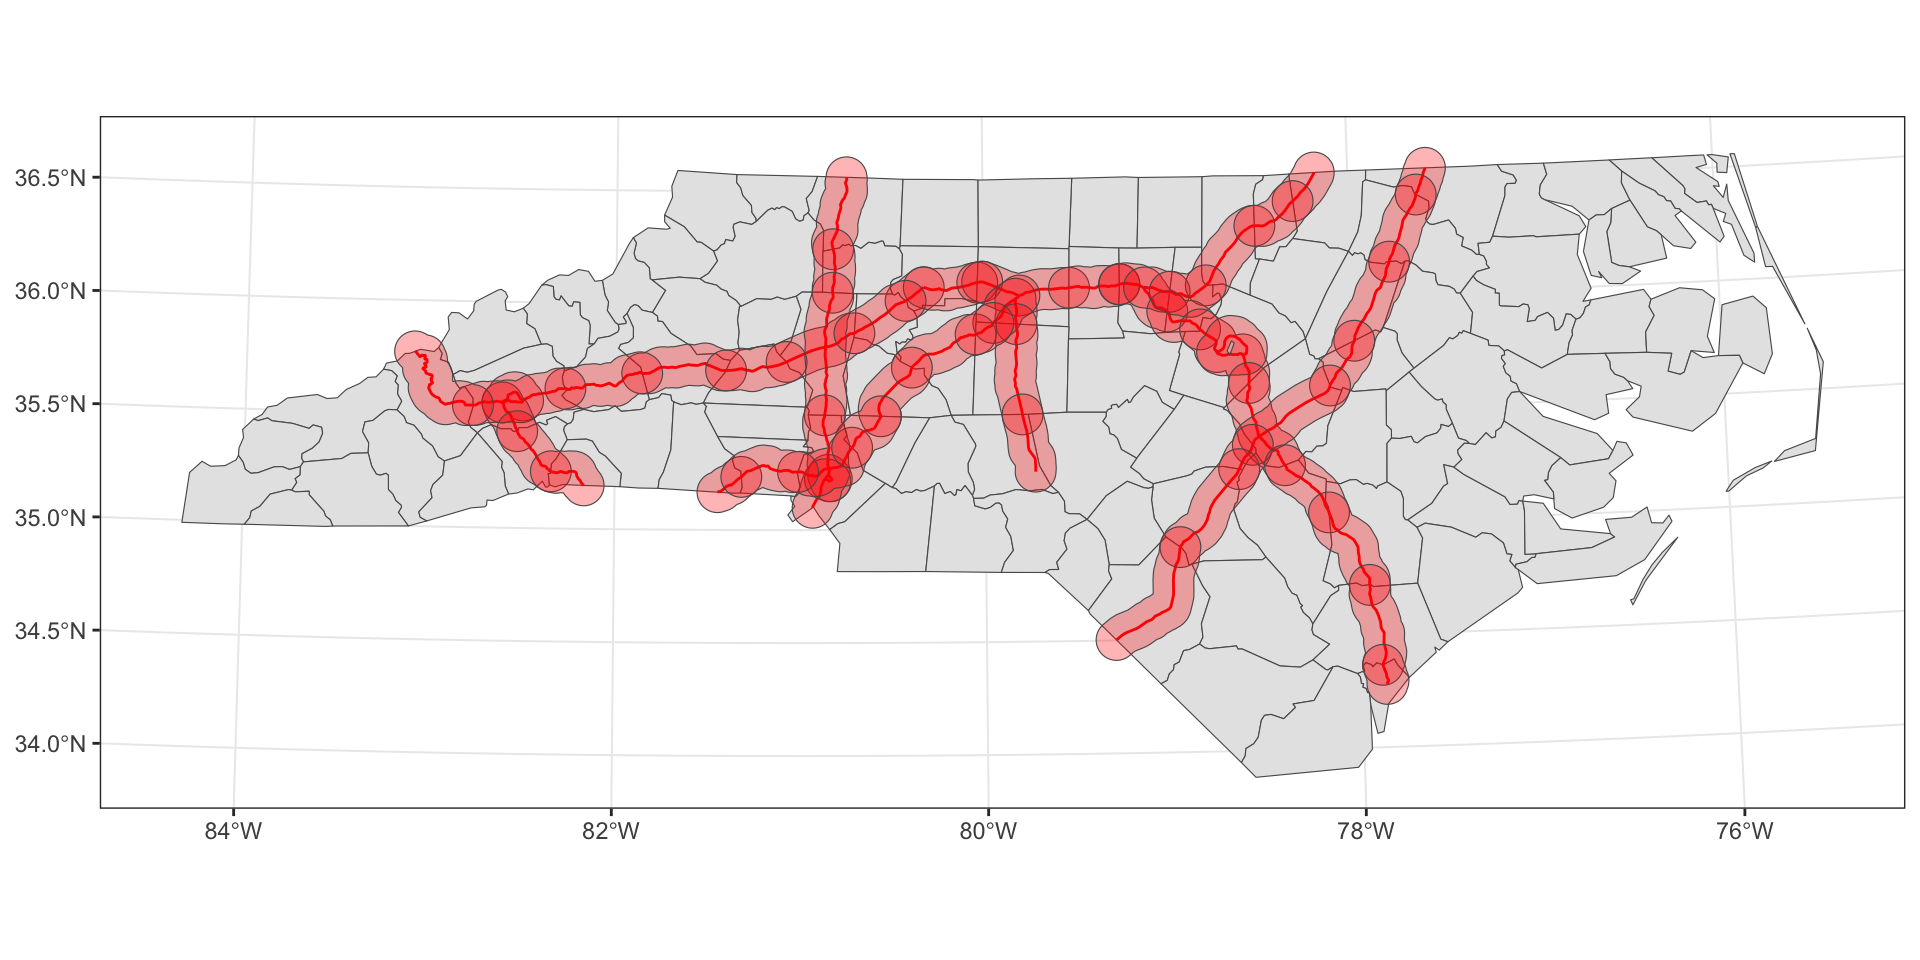
\includegraphics[width=\textwidth]{Lec18_files/figure-beamer/unnamed-chunk-42-1} \end{center}

\end{frame}

\begin{frame}{Posteriors}
\protect\hypertarget{posteriors}{}

\begin{center}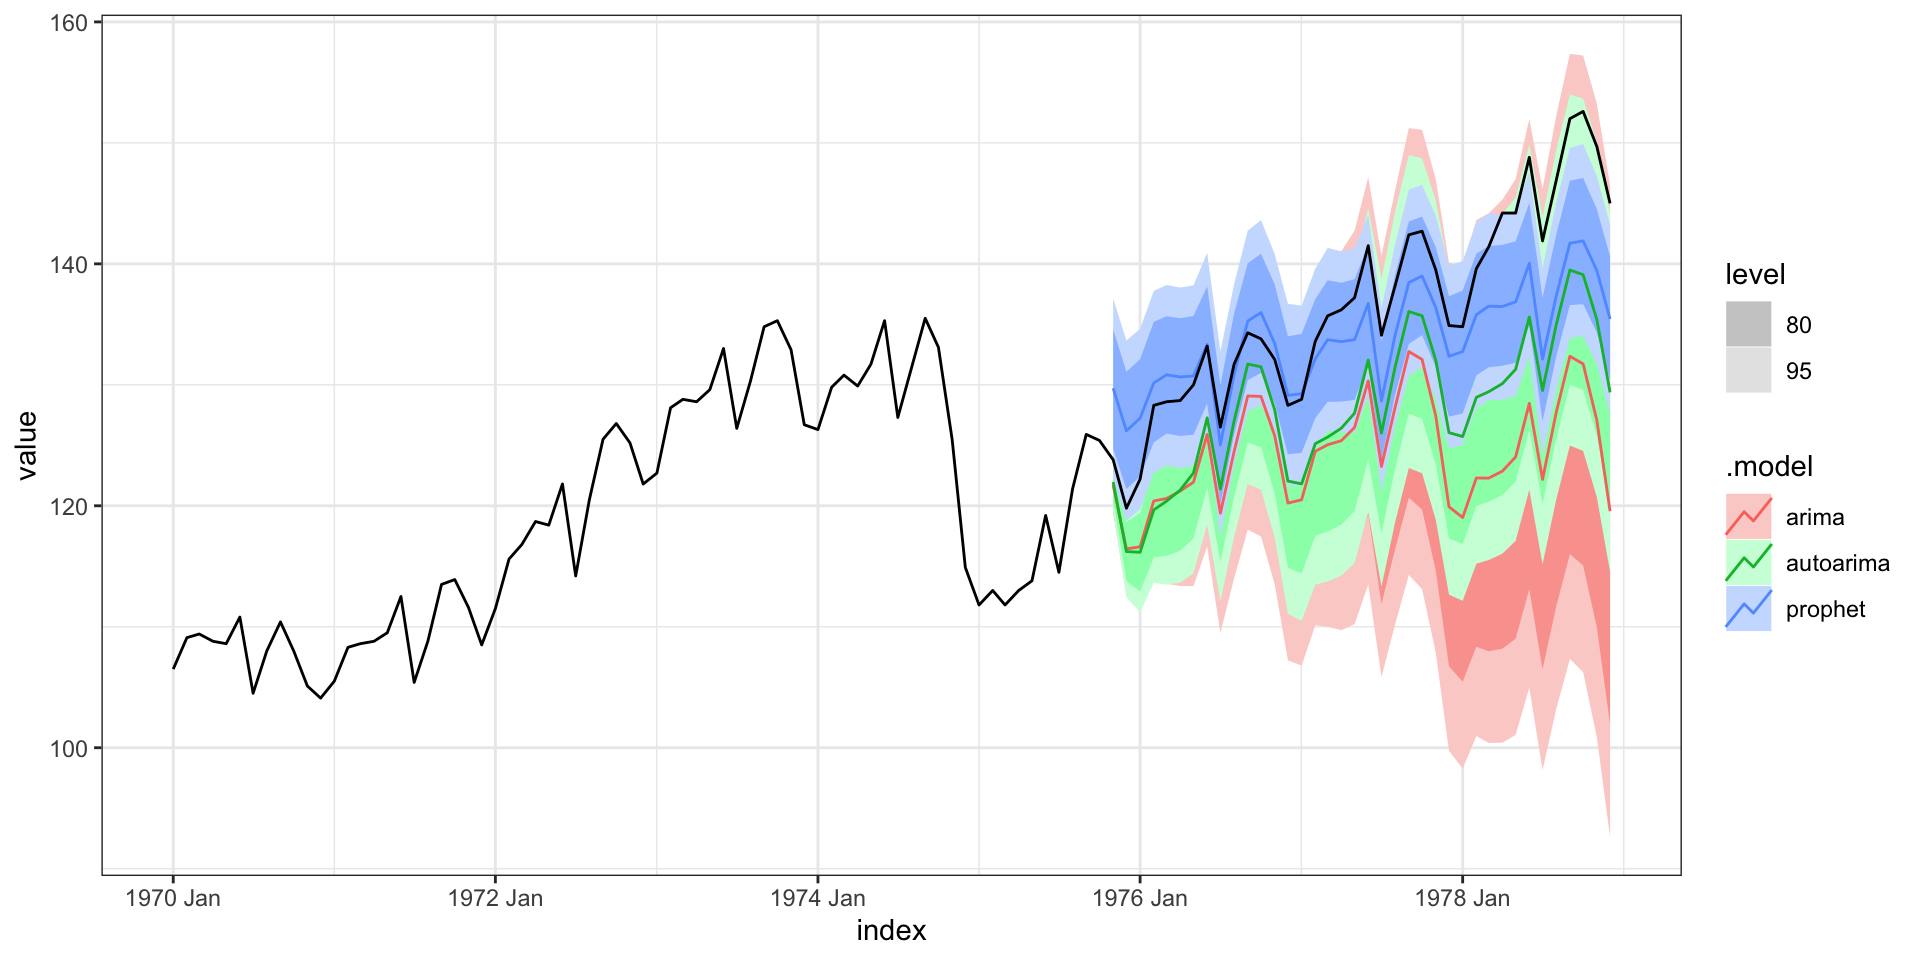
\includegraphics[width=\textwidth]{Lec18_files/figure-beamer/unnamed-chunk-43-1} \end{center}

\end{frame}

\begin{frame}{Predictions}
\protect\hypertarget{predictions-3}{}

\begin{center}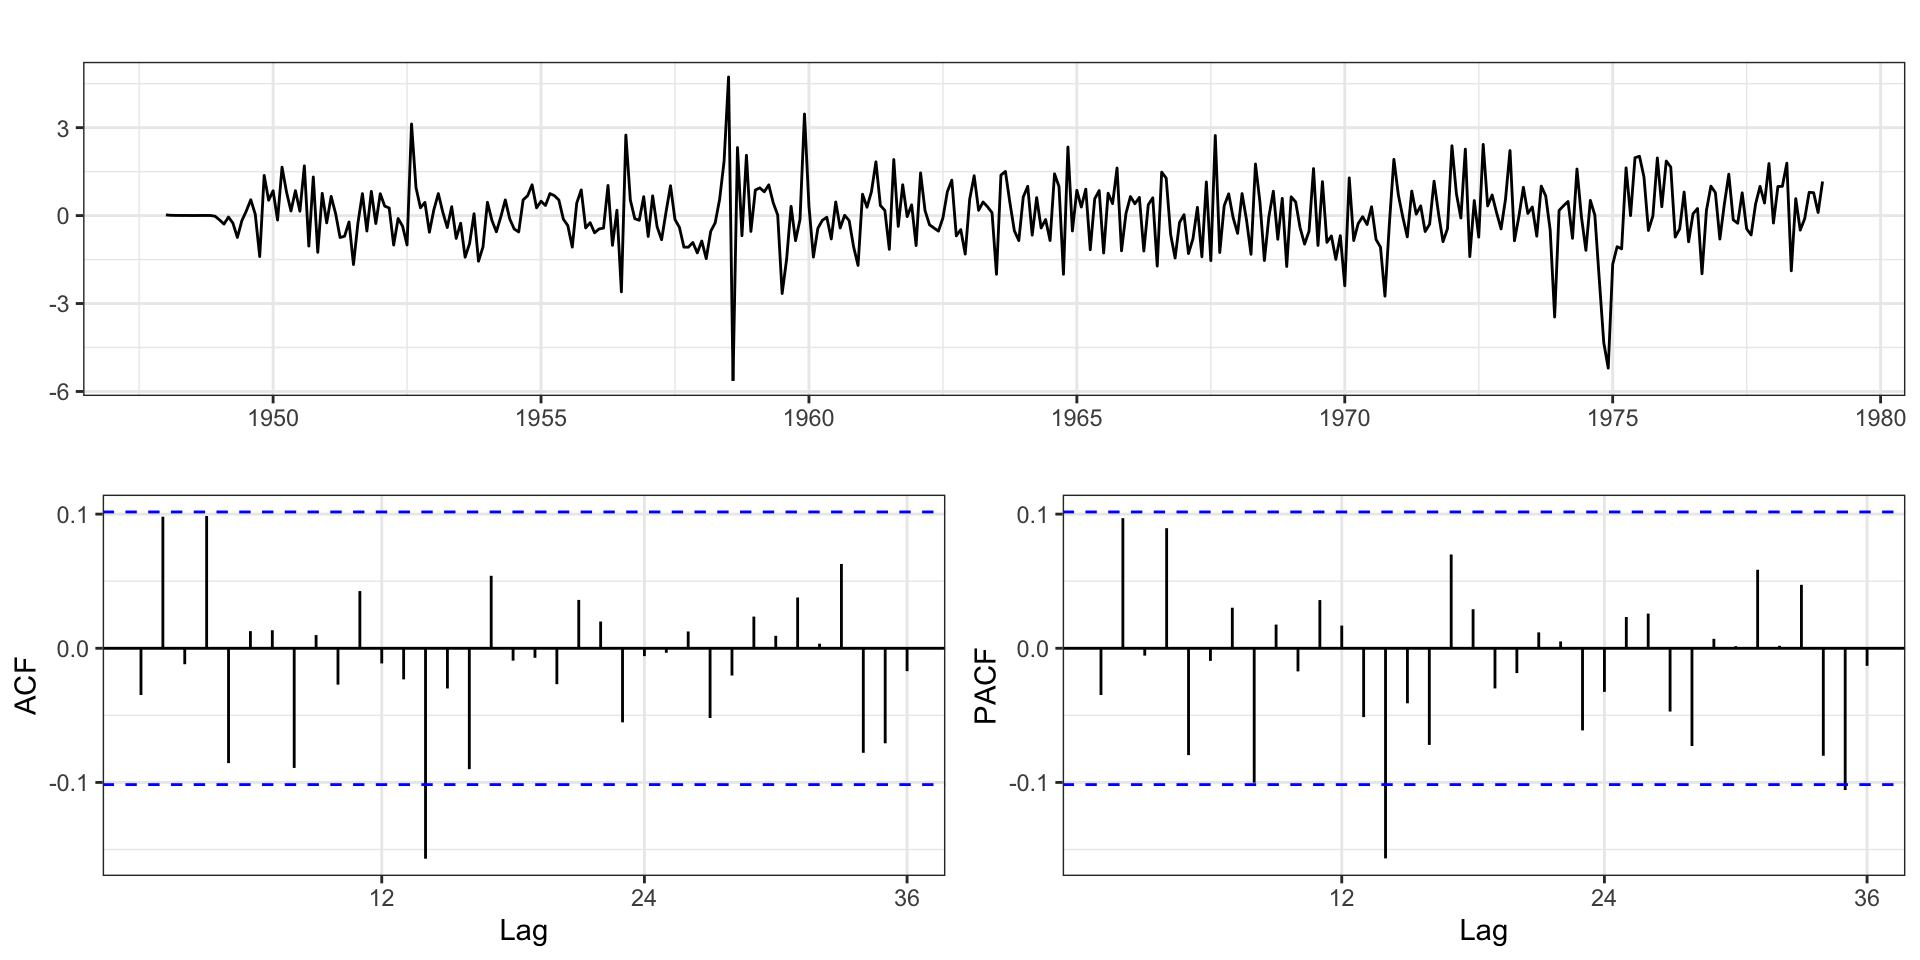
\includegraphics[width=\textwidth]{Lec18_files/figure-beamer/unnamed-chunk-44-1} \end{center}

\end{frame}

\begin{frame}{Predicted vs Observed}
\protect\hypertarget{predicted-vs-observed-1}{}

\begin{center}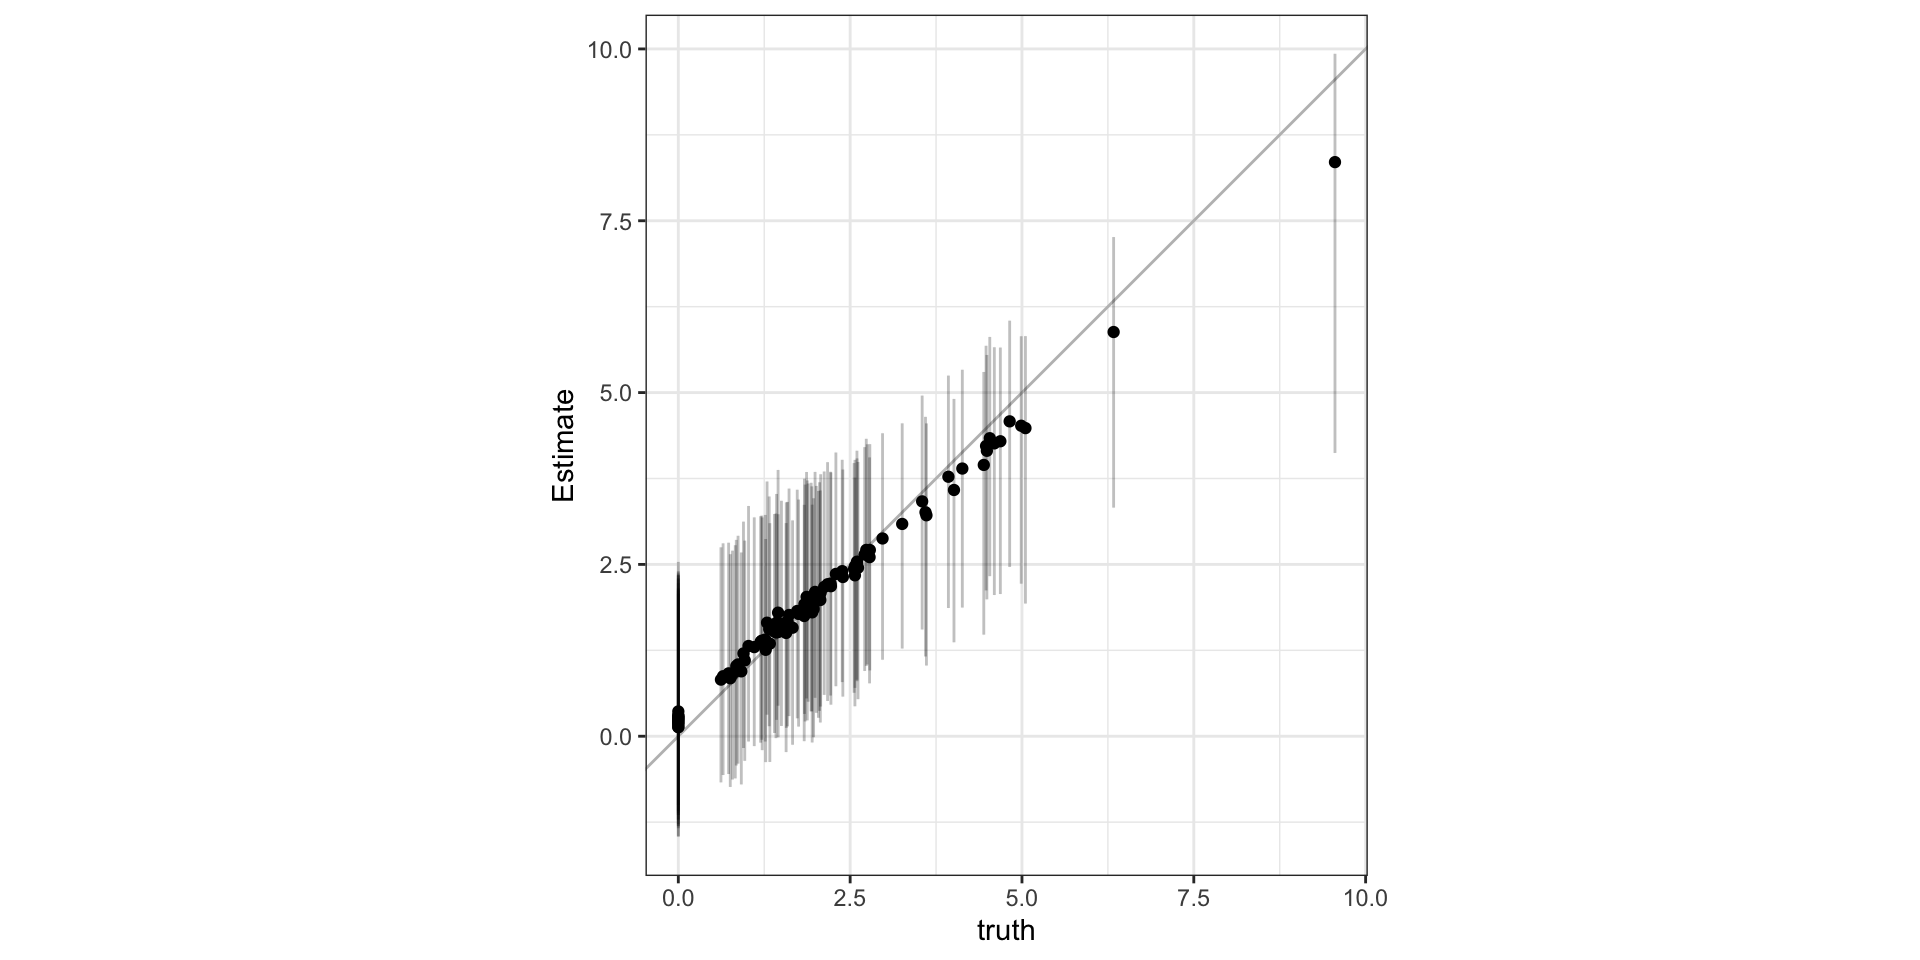
\includegraphics[width=\textwidth]{Lec18_files/figure-beamer/unnamed-chunk-45-1} \end{center}

\end{frame}

\begin{frame}{Predicted vs Observed (cont)}
\protect\hypertarget{predicted-vs-observed-cont}{}

\begin{center}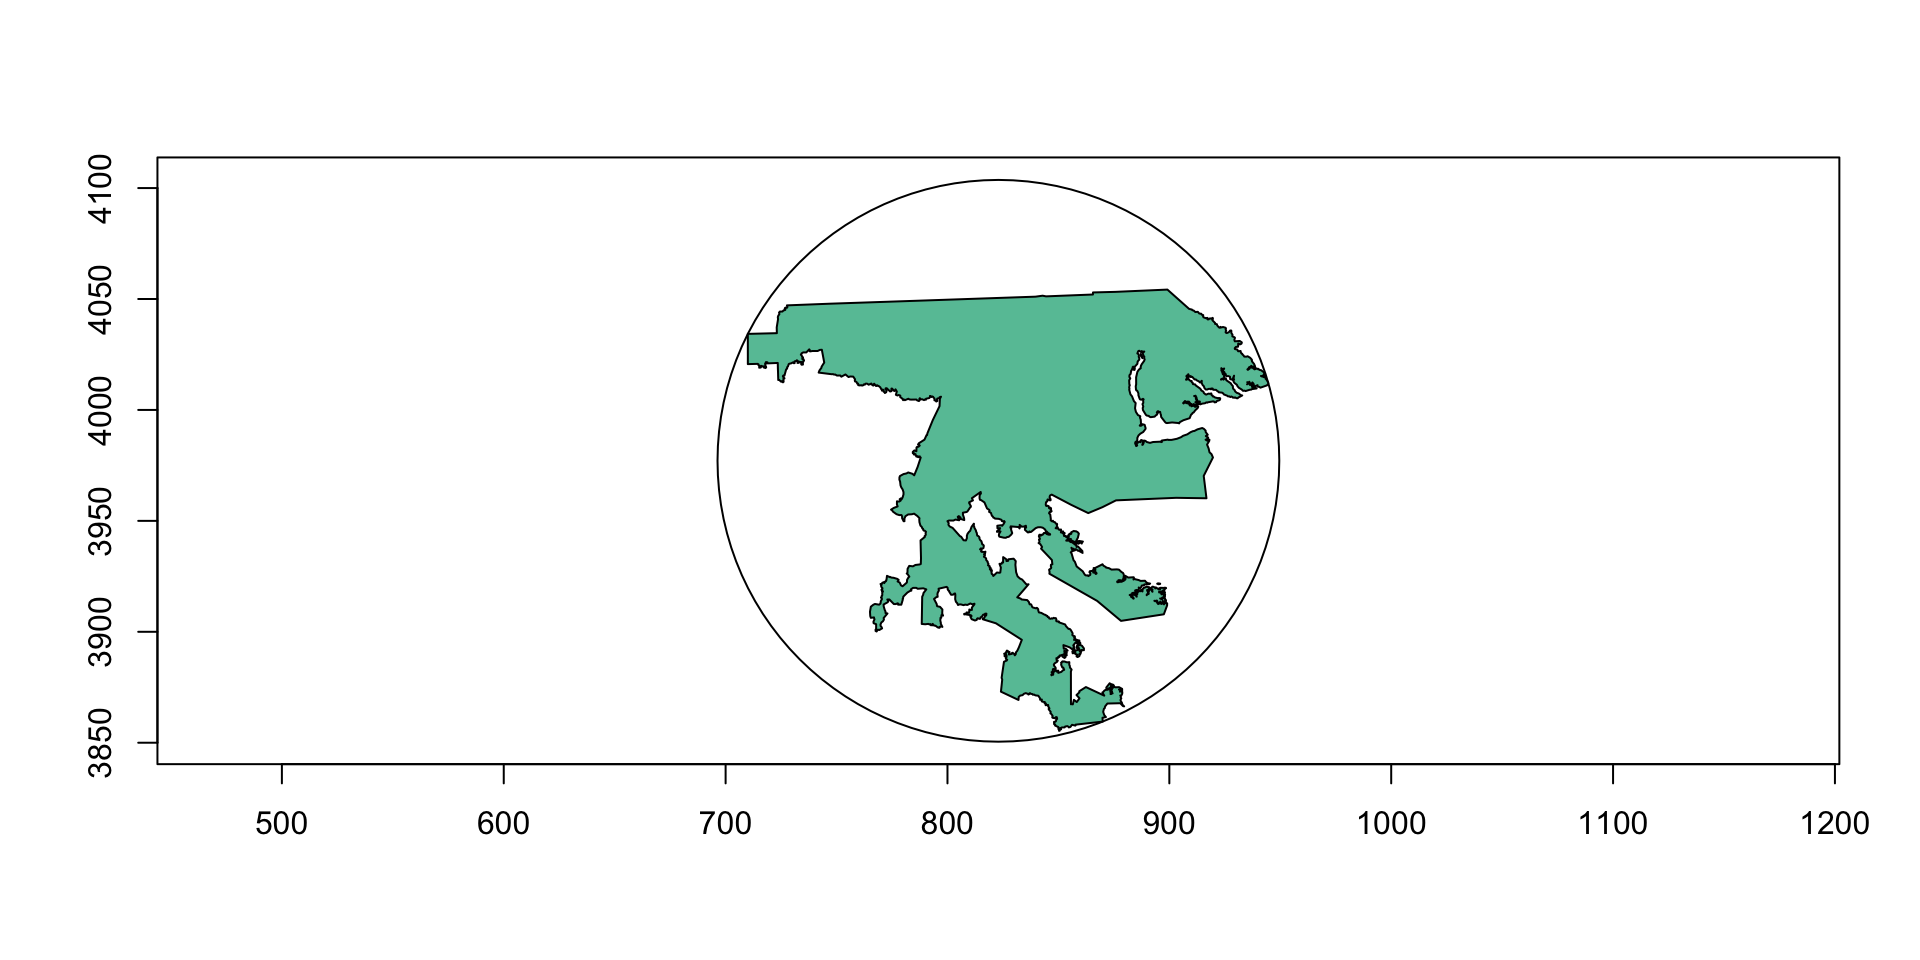
\includegraphics[width=\textwidth]{Lec18_files/figure-beamer/unnamed-chunk-46-1} \end{center}

\end{frame}

\begin{frame}{Model Fit}
\protect\hypertarget{model-fit}{}

\begin{center}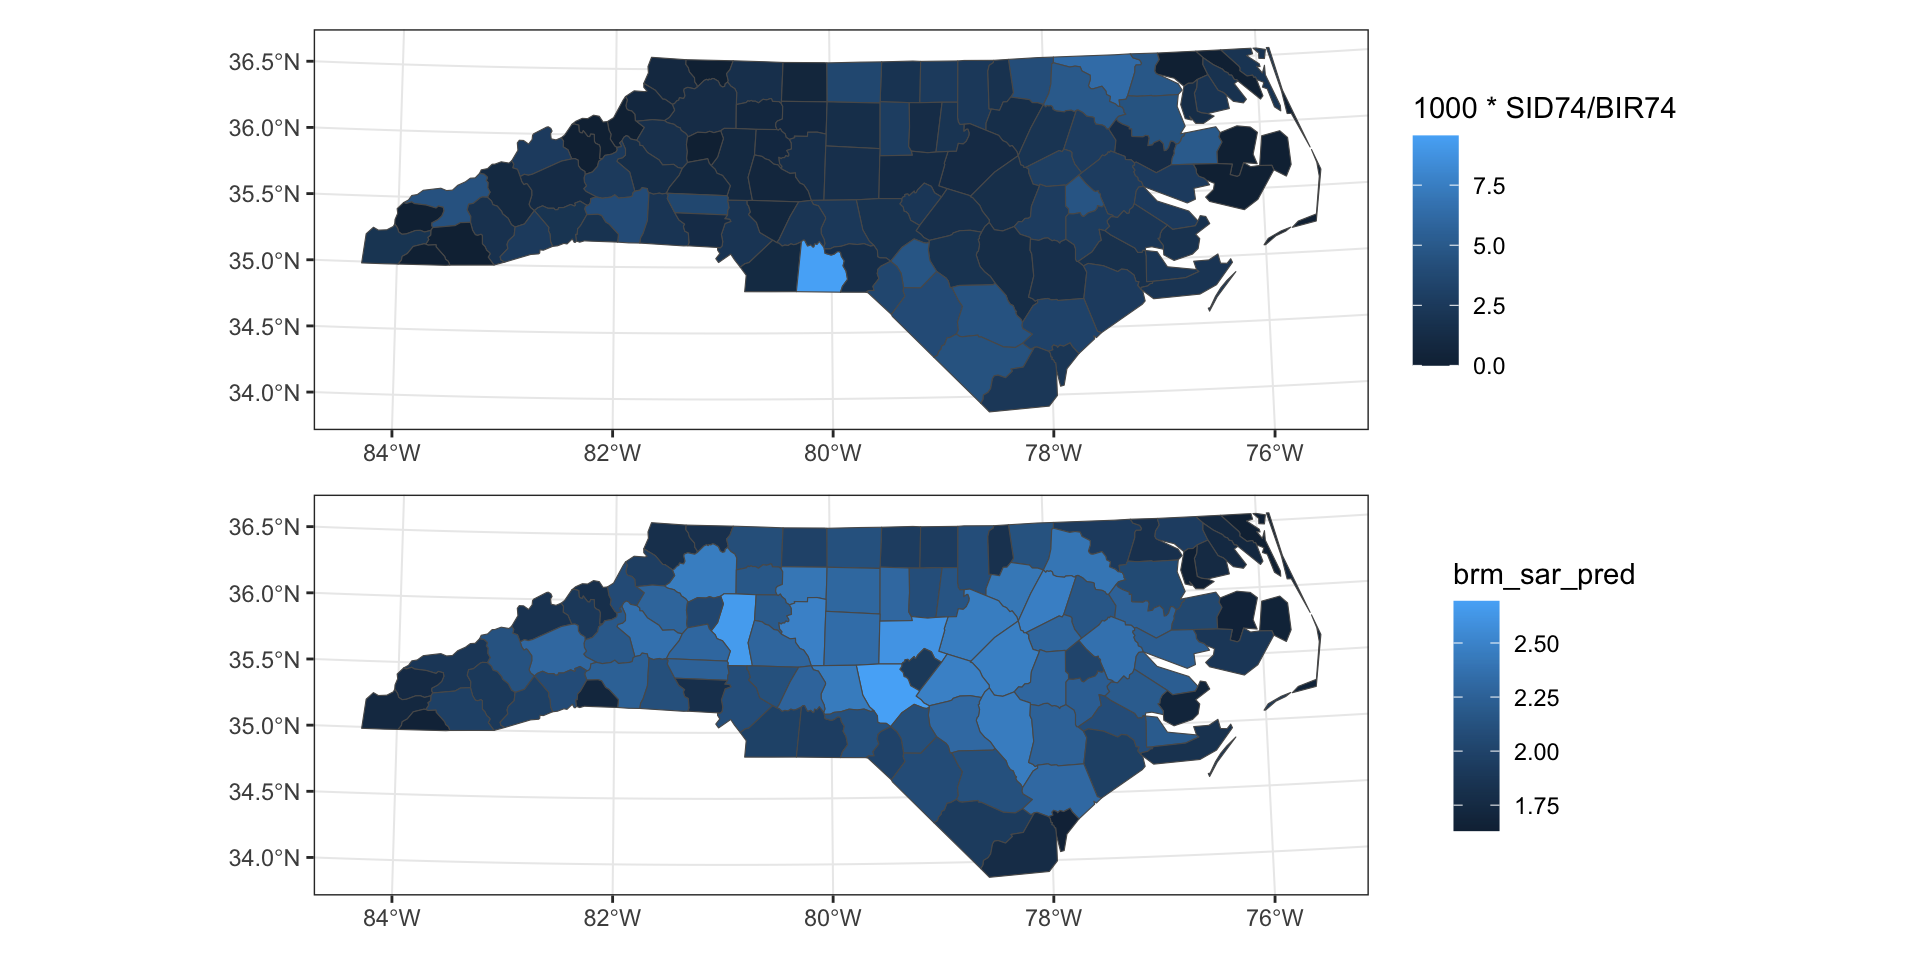
\includegraphics[width=\textwidth]{Lec18_files/figure-beamer/unnamed-chunk-47-1} \end{center}

\end{frame}

\begin{frame}{Model Fit (cont.)}
\protect\hypertarget{model-fit-cont.}{}

\begin{center}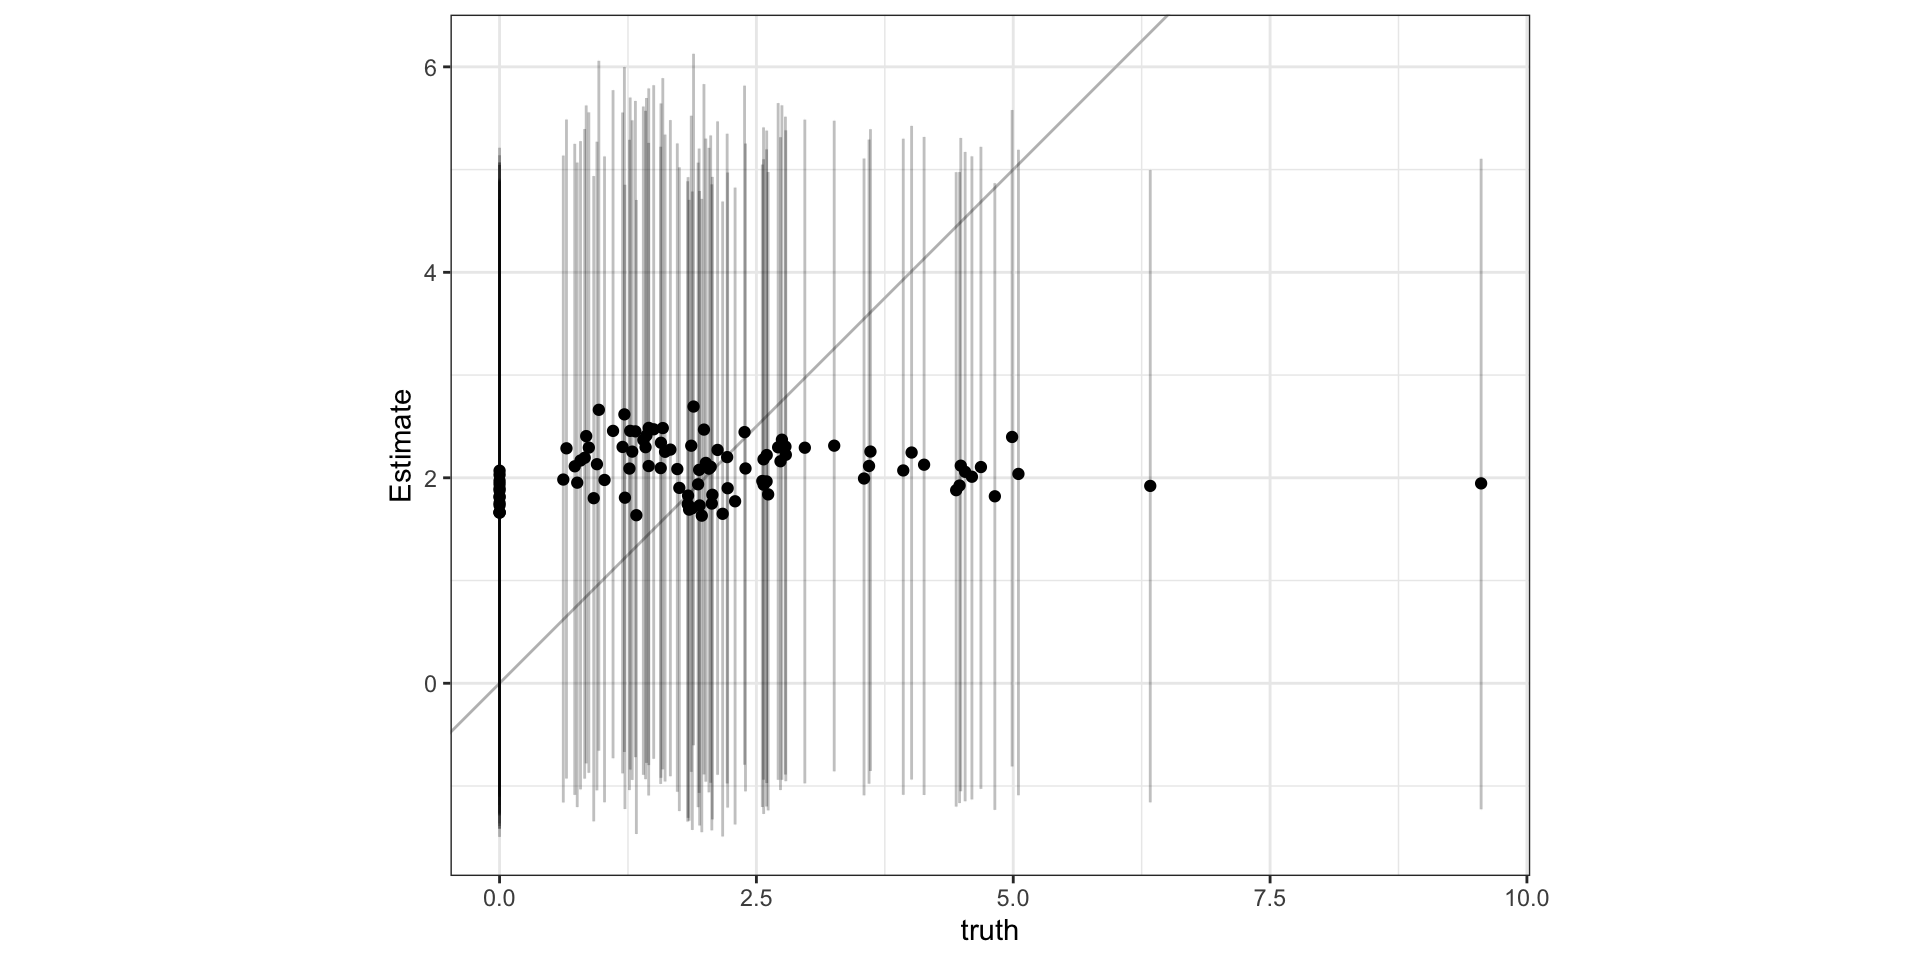
\includegraphics[width=\textwidth]{Lec18_files/figure-beamer/unnamed-chunk-48-1} \end{center}

\end{frame}

\begin{frame}{Model Fit (cont.)}
\protect\hypertarget{model-fit-cont.-1}{}

\begin{center}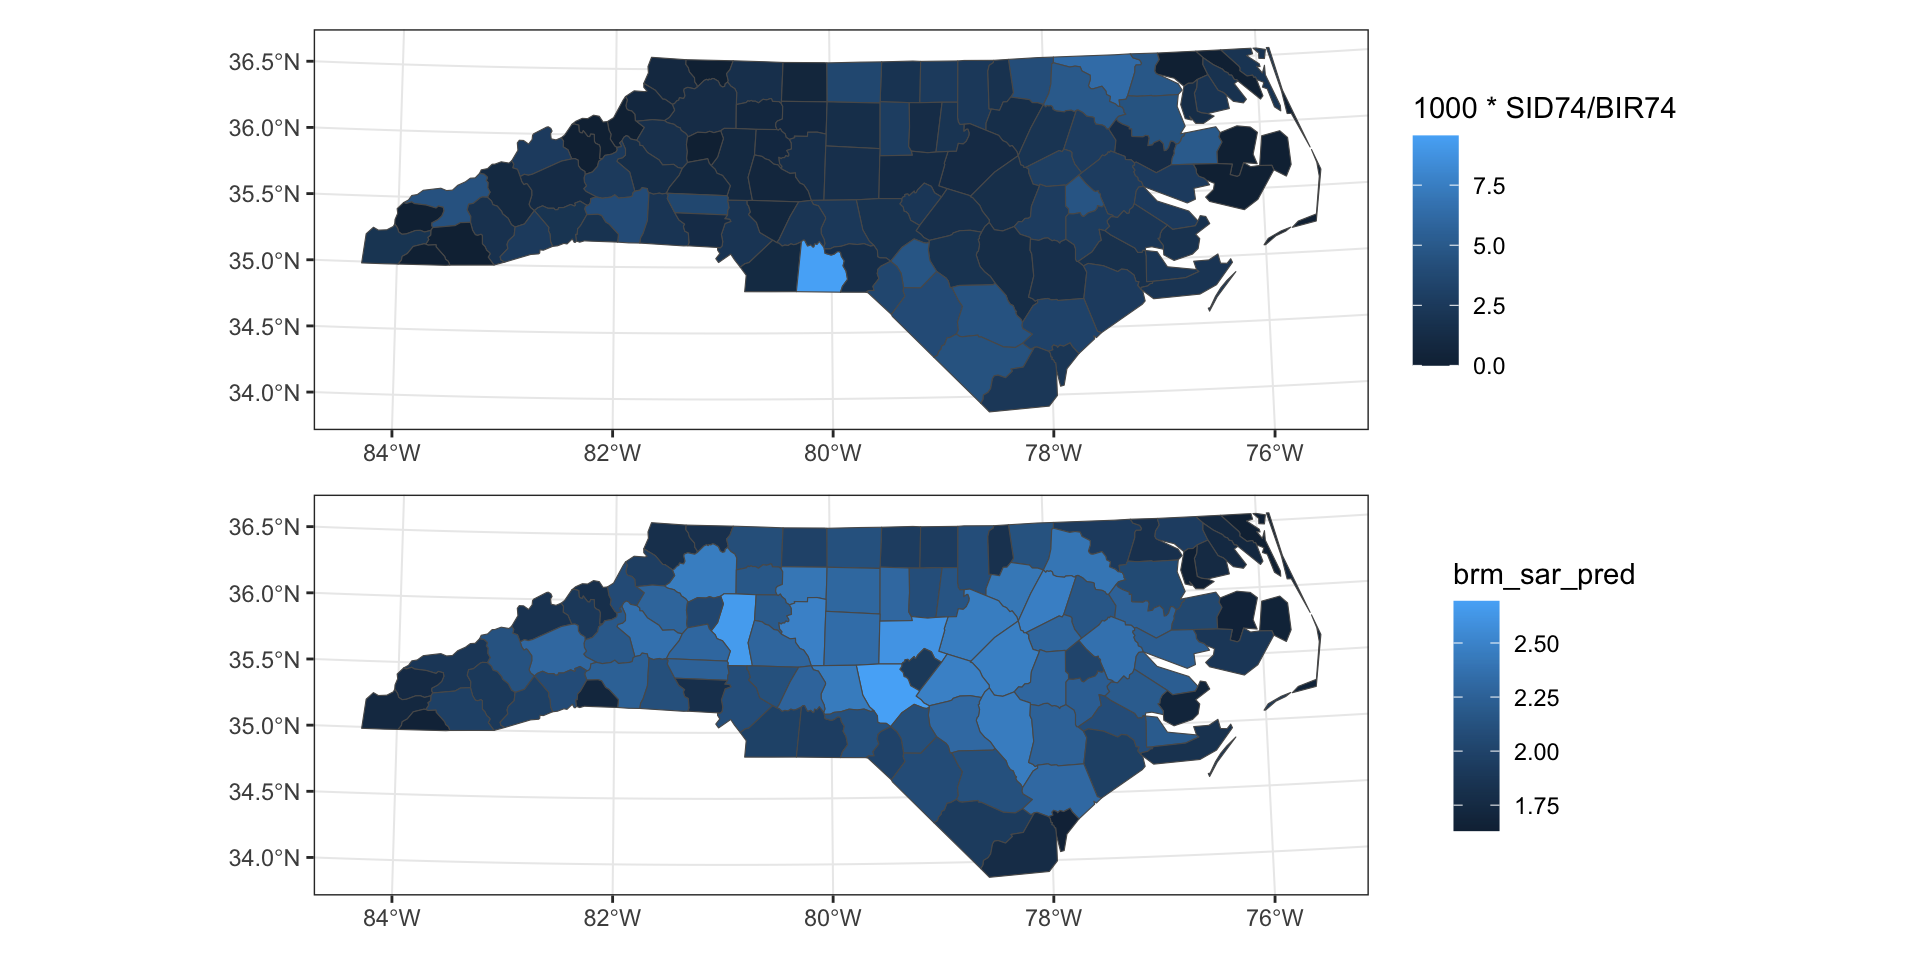
\includegraphics[width=\textwidth]{Lec18_files/figure-beamer/unnamed-chunk-49-1} \end{center}

\end{frame}

\begin{frame}[fragile]{Residuals}
\protect\hypertarget{residuals-1}{}

\scriptoutput

\begin{Shaded}
\begin{Highlighting}[]
\NormalTok{nc =}\StringTok{ }\KeywordTok{mutate}\NormalTok{(nc, }\DataTypeTok{car_log_resid =}\NormalTok{ car_log_pred_post_mean }\OperatorTok{-}\StringTok{ }\KeywordTok{log}\NormalTok{((SID74}\OperatorTok{+}\DecValTok{1}\NormalTok{)}\OperatorTok{/}\NormalTok{BIR74))}

\KeywordTok{ggplot}\NormalTok{(nc, }\KeywordTok{aes}\NormalTok{(}\DataTypeTok{fill=}\NormalTok{car_log_resid)) }\OperatorTok{+}\StringTok{ }\KeywordTok{geom_sf}\NormalTok{()}
\end{Highlighting}
\end{Shaded}

\begin{center}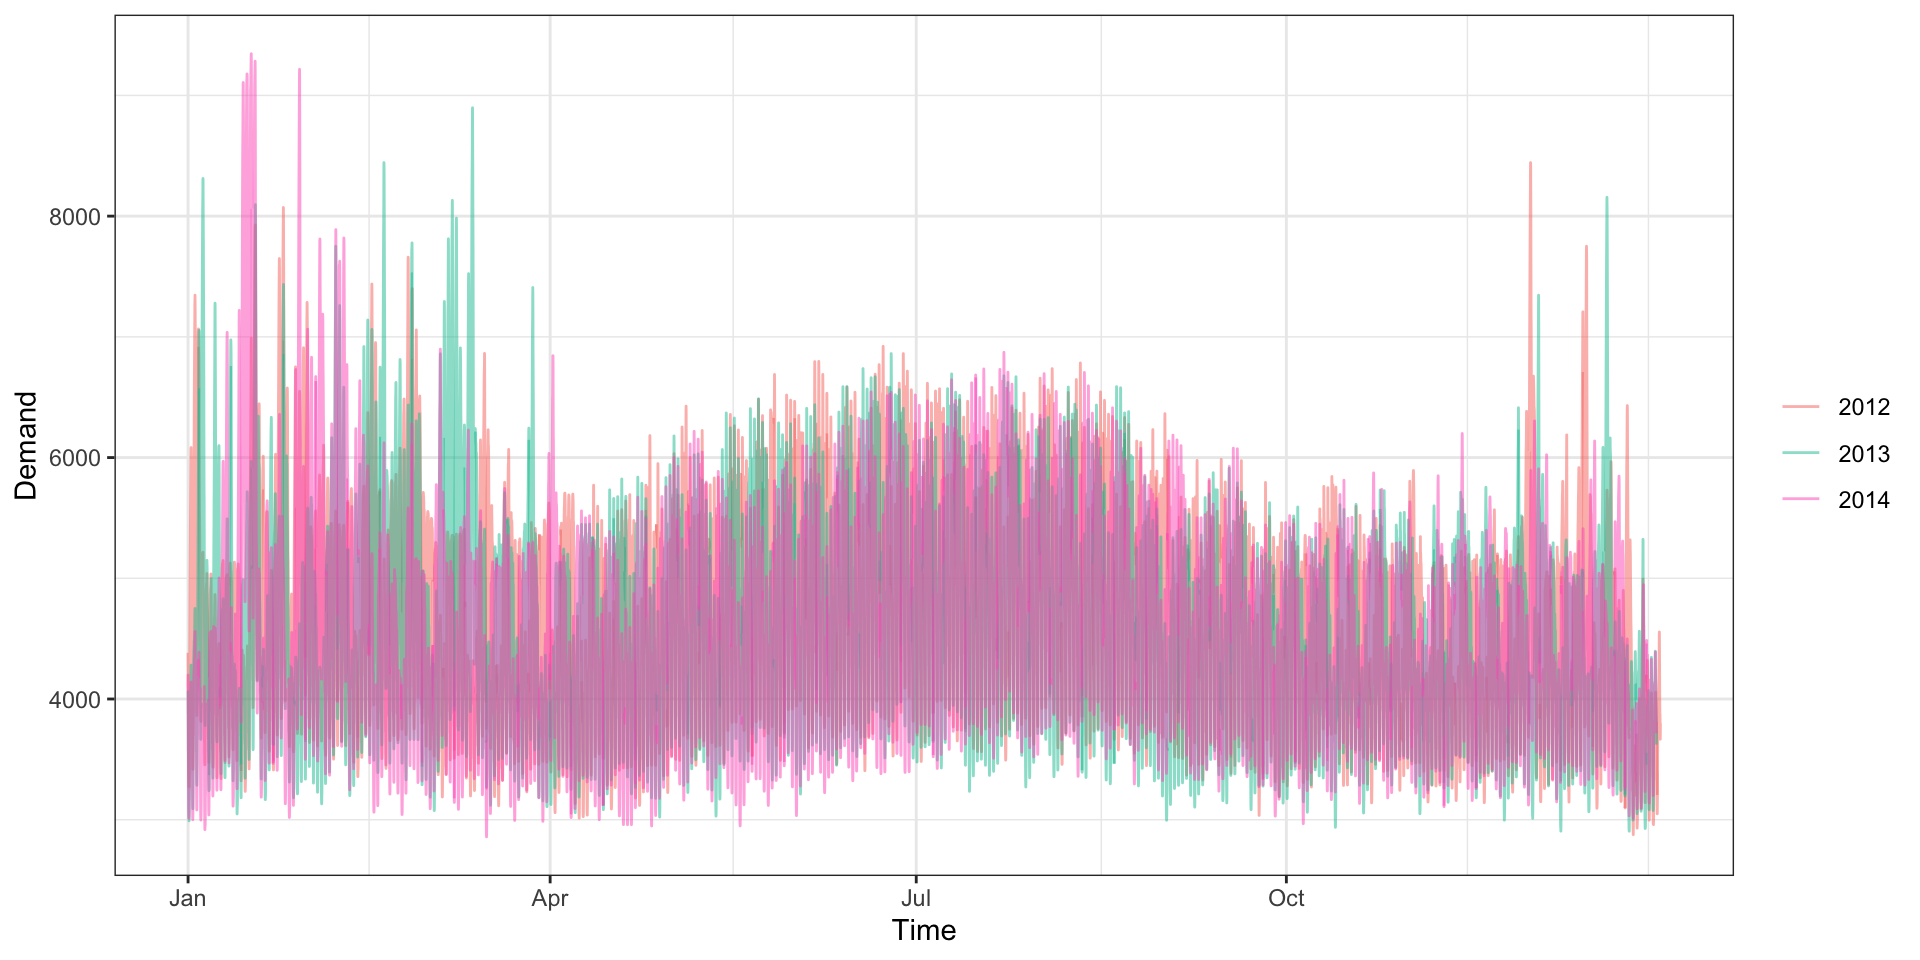
\includegraphics[width=\textwidth]{Lec18_files/figure-beamer/unnamed-chunk-50-1} \end{center}

\begin{Shaded}
\begin{Highlighting}[]
\NormalTok{spdep}\OperatorTok{::}\KeywordTok{moran.test}\NormalTok{(nc}\OperatorTok{$}\NormalTok{car_log_resid, listW)}
\CommentTok{## }
\CommentTok{##  Moran I test under randomisation}
\CommentTok{## }
\CommentTok{## data:  nc$car_log_resid  }
\CommentTok{## weights: listW    }
\CommentTok{## }
\CommentTok{## Moran I statistic standard deviate = -1.1361, p-value = 0.872}
\CommentTok{## alternative hypothesis: greater}
\CommentTok{## sample estimates:}
\CommentTok{## Moran I statistic       Expectation          Variance }
\CommentTok{##      -0.080372616      -0.010101010       0.003826085}
\end{Highlighting}
\end{Shaded}

\end{frame}

\end{document}
